\vspace*{-2.0cm}
\textbf{\Huge Results - Easy environment (1) }
\vspace{1.5cm}
\begin{tikzpicture}[remember picture,overlay]
   \node[anchor=south east,inner sep=20pt] at (current page.south east)
              {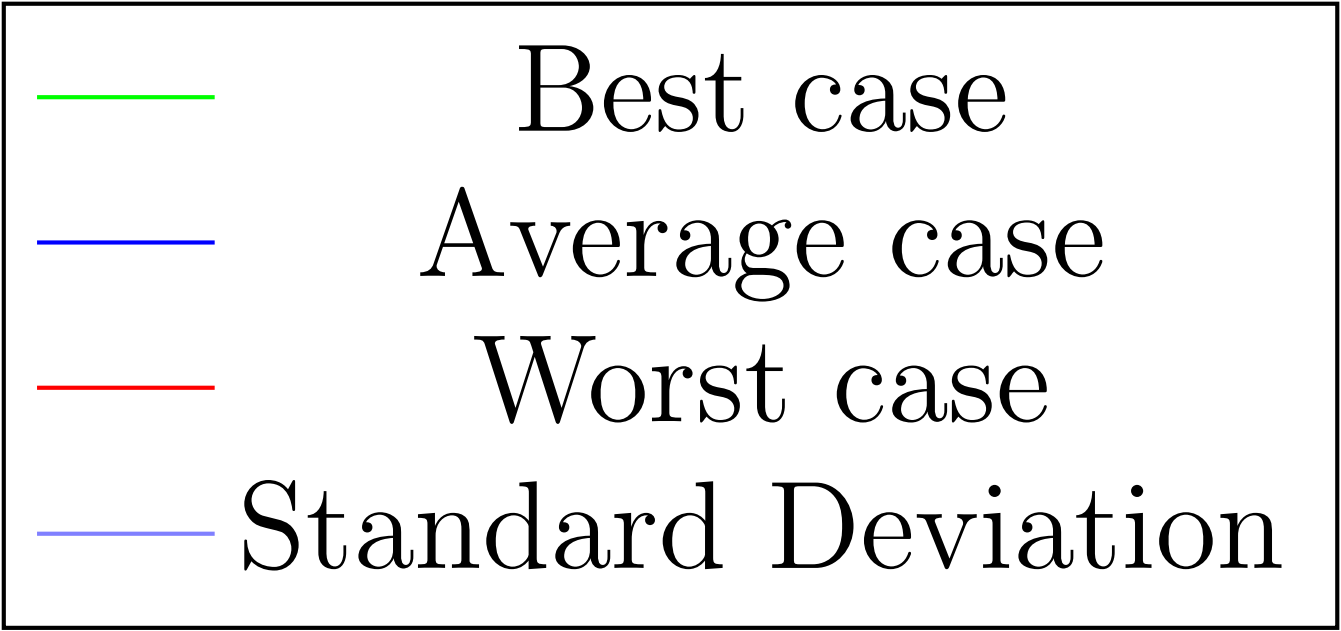
\includegraphics[scale=0.1]{chapters/res/generated_graph_legend.png}};
\end{tikzpicture}

\begin{figure}[H]
\vspace*{-1cm}
	\makebox[\linewidth][c]{%
	\begin{subfigure}[b]{0.7\textwidth}
		\centering
		\resizebox{0.9\linewidth}{!}{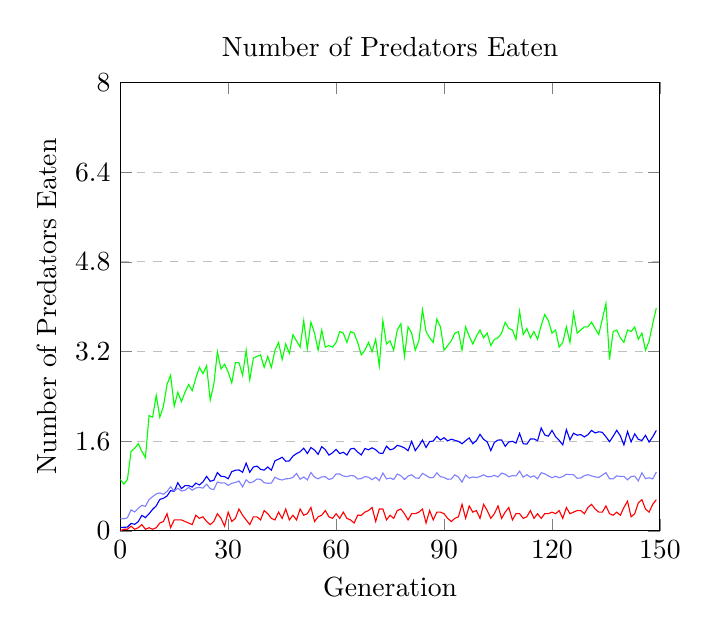
\begin{tikzpicture}
\begin{axis}[
	title={Number of Predators Eaten},
	xlabel={Generation},
	ylabel={Number of Predators Eaten},
	xmin=0, xmax=150,
	ymin=0, ymax=8,
	xtick={0.0,30.0,60.0,90.0,120.0,150.0},
	ytick={0.0,1.6,3.2,4.800000000000001,6.4,8.0},
	ymajorgrids=true,
	grid style=dashed,
]

\addplot[
	color=green,
	]
	coordinates {
	(0,0.9166666666666667)(1,0.8333333333333335)(2,0.9166666666666667)(3,1.4166666666666665)(4,1.4722222222222223)(5,1.5555555555555556)(6,1.4166666666666667)(7,1.3055555555555554)(8,2.0555555555555554)(9,2.027777777777778)(10,2.4166666666666665)(11,2.0277777777777777)(12,2.2222222222222223)(13,2.611111111111111)(14,2.777777777777778)(15,2.222222222222222)(16,2.4722222222222223)(17,2.305555555555556)(18,2.4722222222222223)(19,2.611111111111111)(20,2.5)(21,2.7222222222222228)(22,2.916666666666667)(23,2.8055555555555554)(24,2.944444444444444)(25,2.333333333333333)(26,2.611111111111111)(27,3.194444444444444)(28,2.888888888888889)(29,2.9722222222222228)(30,2.833333333333333)(31,2.6388888888888884)(32,3.0)(33,3.0)(34,2.7777777777777777)(35,3.2222222222222223)(36,2.694444444444444)(37,3.083333333333334)(38,3.1111111111111107)(39,3.138888888888889)(40,2.9166666666666665)(41,3.1111111111111107)(42,2.9166666666666665)(43,3.2222222222222223)(44,3.361111111111111)(45,3.055555555555556)(46,3.3333333333333335)(47,3.166666666666666)(48,3.5)(49,3.3888888888888893)(50,3.2777777777777777)(51,3.75)(52,3.2500000000000004)(53,3.722222222222222)(54,3.527777777777778)(55,3.2222222222222223)(56,3.583333333333333)(57,3.2777777777777786)(58,3.3055555555555554)(59,3.277777777777778)(60,3.3611111111111116)(61,3.5555555555555554)(62,3.5277777777777777)(63,3.361111111111111)(64,3.555555555555556)(65,3.5277777777777777)(66,3.3611111111111107)(67,3.138888888888889)(68,3.222222222222222)(69,3.361111111111111)(70,3.194444444444444)(71,3.4166666666666665)(72,2.944444444444444)(73,3.7500000000000004)(74,3.333333333333333)(75,3.388888888888889)(76,3.2222222222222214)(77,3.583333333333333)(78,3.6944444444444446)(79,3.111111111111111)(80,3.638888888888889)(81,3.5277777777777777)(82,3.2222222222222223)(83,3.388888888888889)(84,3.944444444444444)(85,3.5555555555555554)(86,3.444444444444444)(87,3.361111111111111)(88,3.7777777777777772)(89,3.6388888888888893)(90,3.222222222222222)(91,3.3055555555555554)(92,3.388888888888889)(93,3.5277777777777777)(94,3.5555555555555554)(95,3.222222222222222)(96,3.638888888888889)(97,3.4722222222222223)(98,3.333333333333333)(99,3.4722222222222228)(100,3.5833333333333335)(101,3.444444444444445)(102,3.527777777777778)(103,3.305555555555556)(104,3.4166666666666665)(105,3.4444444444444446)(106,3.5277777777777772)(107,3.722222222222222)(108,3.611111111111111)(109,3.5833333333333335)(110,3.416666666666667)(111,3.9166666666666665)(112,3.5000000000000004)(113,3.611111111111111)(114,3.4444444444444446)(115,3.5555555555555554)(116,3.4166666666666665)(117,3.666666666666667)(118,3.8611111111111107)(119,3.75)(120,3.5277777777777777)(121,3.5833333333333335)(122,3.2777777777777777)(123,3.3611111111111107)(124,3.638888888888889)(125,3.3611111111111116)(126,3.8888888888888893)(127,3.5277777777777777)(128,3.583333333333334)(129,3.638888888888889)(130,3.6388888888888893)(131,3.7222222222222223)(132,3.6111111111111116)(133,3.4999999999999996)(134,3.7777777777777777)(135,4.055555555555555)(136,3.0555555555555554)(137,3.555555555555556)(138,3.5833333333333335)(139,3.4444444444444446)(140,3.361111111111111)(141,3.583333333333333)(142,3.5555555555555554)(143,3.638888888888889)(144,3.416666666666667)(145,3.527777777777778)(146,3.222222222222222)(147,3.388888888888889)(148,3.6944444444444446)(149,3.972222222222222)
	};
\addplot[
	color=blue,
	]
	coordinates {
	(0,0.06134259259259259)(1,0.0625)(2,0.06712962962962962)(3,0.13194444444444445)(4,0.11574074074074076)(5,0.16319444444444442)(6,0.2743055555555555)(7,0.23611111111111113)(8,0.30439814814814814)(9,0.38310185185185186)(10,0.4456018518518518)(11,0.560185185185185)(12,0.5810185185185186)(13,0.6203703703703703)(14,0.716435185185185)(15,0.704861111111111)(16,0.8587962962962964)(17,0.7546296296296297)(18,0.8055555555555557)(19,0.8055555555555555)(20,0.78125)(21,0.8506944444444444)(22,0.8182870370370371)(23,0.8738425925925926)(24,0.9710648148148148)(25,0.8842592592592591)(26,0.9016203703703702)(27,1.0381944444444446)(28,0.9733796296296293)(29,0.9675925925925927)(30,0.9282407407407408)(31,1.0555555555555556)(32,1.0810185185185184)(33,1.0856481481481481)(34,1.0451388888888888)(35,1.207175925925926)(36,1.0439814814814814)(37,1.1388888888888888)(38,1.1550925925925923)(39,1.097222222222222)(40,1.0833333333333333)(41,1.1388888888888888)(42,1.0810185185185188)(43,1.25)(44,1.2777777777777777)(45,1.3136574074074072)(46,1.2418981481481481)(47,1.2476851851851851)(48,1.3333333333333335)(49,1.3784722222222223)(50,1.4108796296296295)(51,1.4733796296296298)(52,1.378472222222222)(53,1.4861111111111112)(54,1.4409722222222223)(55,1.3645833333333335)(56,1.502314814814815)(57,1.4479166666666667)(58,1.3506944444444444)(59,1.3923611111111112)(60,1.4525462962962963)(61,1.3784722222222223)(62,1.4016203703703705)(63,1.351851851851852)(64,1.4606481481481481)(65,1.4710648148148147)(66,1.4050925925925928)(67,1.3541666666666665)(68,1.46875)(69,1.4456018518518519)(70,1.4814814814814814)(71,1.4467592592592593)(72,1.386574074074074)(73,1.380787037037037)(74,1.5092592592592593)(75,1.4444444444444442)(76,1.4641203703703705)(77,1.525462962962963)(78,1.5081018518518516)(79,1.4791666666666667)(80,1.4293981481481481)(81,1.597222222222222)(82,1.4305555555555554)(83,1.5173611111111112)(84,1.6192129629629635)(85,1.4872685185185186)(86,1.5925925925925926)(87,1.6018518518518519)(88,1.685185185185185)(89,1.6203703703703702)(90,1.662037037037037)(91,1.6041666666666667)(92,1.6354166666666665)(93,1.6145833333333337)(94,1.5972222222222223)(95,1.5532407407407405)(96,1.6087962962962963)(97,1.6574074074074074)(98,1.5543981481481484)(99,1.6099537037037037)(100,1.721064814814815)(101,1.6319444444444444)(102,1.5868055555555554)(103,1.4317129629629628)(104,1.5787037037037035)(105,1.6192129629629635)(106,1.6215277777777777)(107,1.508101851851852)(108,1.585648148148148)(109,1.597222222222222)(110,1.5659722222222219)(111,1.7384259259259258)(112,1.5543981481481481)(113,1.5462962962962963)(114,1.6377314814814816)(115,1.6400462962962965)(116,1.6087962962962965)(117,1.8344907407407405)(118,1.710648148148148)(119,1.6886574074074074)(120,1.7916666666666665)(121,1.6805555555555554)(122,1.6145833333333335)(123,1.5335648148148149)(124,1.8067129629629632)(125,1.6249999999999998)(126,1.7418981481481481)(127,1.7060185185185186)(128,1.7175925925925926)(129,1.6747685185185188)(130,1.7164351851851856)(131,1.791666666666667)(132,1.7465277777777775)(133,1.7673611111111112)(134,1.7569444444444444)(135,1.6782407407407405)(136,1.590277777777778)(137,1.6851851851851853)(138,1.7939814814814816)(139,1.6944444444444442)(140,1.5324074074074074)(141,1.7719907407407407)(142,1.5868055555555556)(143,1.7303240740740737)(144,1.6319444444444442)(145,1.6122685185185184)(146,1.7037037037037037)(147,1.5833333333333333)(148,1.6770833333333333)(149,1.7905092592592593)
	};
\addplot[
	color=red,
	]
	coordinates {
	(0,0.0)(1,0.027777777777777776)(2,0.027777777777777776)(3,0.08333333333333333)(4,0.027777777777777776)(5,0.05555555555555555)(6,0.1111111111111111)(7,0.027777777777777776)(8,0.05555555555555555)(9,0.027777777777777776)(10,0.05555555555555555)(11,0.1388888888888889)(12,0.16666666666666669)(13,0.3055555555555556)(14,0.05555555555555555)(15,0.19444444444444445)(16,0.19444444444444445)(17,0.19444444444444442)(18,0.16666666666666666)(19,0.1388888888888889)(20,0.1111111111111111)(21,0.27777777777777773)(22,0.22222222222222224)(23,0.25)(24,0.16666666666666666)(25,0.1111111111111111)(26,0.16666666666666666)(27,0.3055555555555555)(28,0.2222222222222222)(29,0.08333333333333333)(30,0.33333333333333337)(31,0.16666666666666669)(32,0.2222222222222222)(33,0.38888888888888895)(34,0.2777777777777778)(35,0.19444444444444445)(36,0.1111111111111111)(37,0.25)(38,0.24999999999999997)(39,0.19444444444444448)(40,0.36111111111111116)(41,0.3055555555555555)(42,0.22222222222222227)(43,0.19444444444444442)(44,0.33333333333333337)(45,0.2222222222222222)(46,0.38888888888888884)(47,0.19444444444444442)(48,0.2777777777777778)(49,0.19444444444444442)(50,0.38888888888888895)(51,0.2777777777777778)(52,0.3055555555555556)(53,0.4166666666666667)(54,0.16666666666666666)(55,0.25)(56,0.2777777777777778)(57,0.36111111111111116)(58,0.25)(59,0.2222222222222222)(60,0.3055555555555555)(61,0.2222222222222222)(62,0.33333333333333337)(63,0.2222222222222222)(64,0.19444444444444445)(65,0.1388888888888889)(66,0.2777777777777778)(67,0.2777777777777778)(68,0.33333333333333337)(69,0.36111111111111116)(70,0.41666666666666674)(71,0.16666666666666666)(72,0.38888888888888895)(73,0.38888888888888895)(74,0.19444444444444445)(75,0.2777777777777778)(76,0.2222222222222222)(77,0.36111111111111116)(78,0.38888888888888895)(79,0.3055555555555556)(80,0.19444444444444445)(81,0.3055555555555556)(82,0.3055555555555556)(83,0.33333333333333337)(84,0.38888888888888895)(85,0.1388888888888889)(86,0.36111111111111105)(87,0.19444444444444445)(88,0.33333333333333337)(89,0.33333333333333337)(90,0.3055555555555555)(91,0.22222222222222224)(92,0.16666666666666669)(93,0.2222222222222222)(94,0.25)(95,0.4722222222222222)(96,0.2222222222222222)(97,0.4444444444444445)(98,0.33333333333333337)(99,0.36111111111111116)(100,0.2222222222222222)(101,0.4722222222222222)(102,0.36111111111111116)(103,0.22222222222222224)(104,0.3055555555555556)(105,0.4444444444444445)(106,0.2222222222222222)(107,0.3333333333333333)(108,0.41666666666666674)(109,0.19444444444444442)(110,0.3055555555555556)(111,0.3055555555555556)(112,0.2222222222222222)(113,0.25)(114,0.36111111111111116)(115,0.22222222222222224)(116,0.3055555555555556)(117,0.22222222222222224)(118,0.3055555555555555)(119,0.3055555555555556)(120,0.33333333333333337)(121,0.3055555555555556)(122,0.36111111111111116)(123,0.22222222222222224)(124,0.41666666666666663)(125,0.3055555555555556)(126,0.33333333333333337)(127,0.36111111111111116)(128,0.36111111111111116)(129,0.3055555555555556)(130,0.41666666666666674)(131,0.4722222222222223)(132,0.38888888888888895)(133,0.33333333333333337)(134,0.33333333333333337)(135,0.44444444444444436)(136,0.3055555555555556)(137,0.2777777777777778)(138,0.33333333333333337)(139,0.2777777777777778)(140,0.41666666666666674)(141,0.5277777777777778)(142,0.25)(143,0.3055555555555555)(144,0.5000000000000001)(145,0.5555555555555556)(146,0.38888888888888884)(147,0.33333333333333337)(148,0.47222222222222227)(149,0.5555555555555557)
	};
\addplot[
	color=blue!50,
	]
	coordinates {
	(0,0.22321045150736538)(1,0.21307115581815605)(2,0.234038879917527)(3,0.37427485450144754)(4,0.33624414663585406)(5,0.40051810561928763)(6,0.4544411189604483)(7,0.436614378113725)(8,0.5571213038275963)(9,0.6093692895454634)(10,0.6579663129087959)(11,0.6769468790069775)(12,0.6521088969732397)(13,0.7043527918385674)(14,0.7862418407018714)(15,0.7089847770376726)(16,0.7595879765906958)(17,0.7097683712172996)(18,0.7247915555886776)(19,0.7743396229546845)(20,0.7238812768095757)(21,0.7643394433011678)(22,0.774162527914995)(23,0.7623726637616809)(24,0.8328498977925949)(25,0.7523538055455742)(26,0.73399111866759)(27,0.8710086748354838)(28,0.8524751361693022)(29,0.856539341920678)(30,0.8099154704221928)(31,0.8486898036385229)(32,0.862387448164029)(33,0.889176355248584)(34,0.7836345370232459)(35,0.9114105939553477)(36,0.8551517017703595)(37,0.8757538971827888)(38,0.9249452044520576)(39,0.9181317019352095)(40,0.8582866125284323)(41,0.8492238715833101)(42,0.8502959222954733)(43,0.9567608832713115)(44,0.9222218245255094)(45,0.9063250594350568)(46,0.9292308836141749)(47,0.9306203828186339)(48,0.9539083683255686)(49,1.0232092234813204)(50,0.9201576506188784)(51,0.9613247077730941)(52,0.9082505324357465)(53,1.040460748892688)(54,0.9583244223476725)(55,0.9278695091768099)(56,0.9627512197468809)(57,0.9652569235554224)(58,0.9160268014057982)(59,0.935579481982368)(60,1.01516652784045)(61,1.0132410985505067)(62,0.9768871334813395)(63,0.9665996166527089)(64,0.9860507106856055)(65,0.9807466231996467)(66,0.9248051732662264)(67,0.9321443125930113)(68,0.9668511186787326)(69,0.9574805204700731)(70,0.9122346482028081)(71,0.9555470298311424)(72,0.8962486341584958)(73,1.0323592705612057)(74,0.9266959074015504)(75,0.9418735154773388)(76,0.9146761510238581)(77,1.0130522145218621)(78,0.9830573121846689)(79,0.9157101949997585)(80,0.9774743496278252)(81,0.9999902657480054)(82,0.9452280287274991)(83,0.9356085622064394)(84,1.0259046058392374)(85,0.9880380845352796)(86,0.947566188617334)(87,0.9493945457251167)(88,1.0342328462453652)(89,0.967153871844688)(90,0.950936363164399)(91,0.9201765397986473)(92,0.9235943061664474)(93,0.9990063778875322)(94,0.957974016027371)(95,0.8695771616896256)(96,0.9959498567118912)(97,0.9405133225104956)(98,0.9621035655151938)(99,0.9489117159598254)(100,0.9694362229070564)(101,0.9990055116107914)(102,0.9648640777408772)(103,0.9659119682655598)(104,0.9906275218793971)(105,0.9615951338185366)(106,1.0296823622091795)(107,1.0100038929299202)(108,0.964801406292636)(109,0.9846059805629548)(110,0.9795904553103706)(111,1.0651488080373694)(112,0.9566920813929177)(113,1.0024264206932618)(114,0.9558106189663003)(115,0.9815242681110105)(116,0.9274328869053938)(117,1.0368010802301286)(118,1.0177761558420195)(119,0.9811193297745942)(120,0.9467359199077714)(121,0.9736722202999724)(122,0.9469897062000674)(123,0.9676834087391173)(124,1.0098888922788969)(125,1.001581965419476)(126,1.0017195668329708)(127,0.9373917674025224)(128,0.9428099430481853)(129,0.984476851573527)(130,1.0025653246595172)(131,0.9795362708864437)(132,0.9630823432252511)(133,0.9505018223290455)(134,0.9952469305587185)(135,1.038254265109217)(136,0.9291952418362378)(137,0.9271642917831885)(138,0.981053899372655)(139,0.9696358332824201)(140,0.9709020683684676)(141,0.9100155932664445)(142,0.9689896842566308)(143,0.9761691845365206)(144,0.8913265145528558)(145,1.036922900295025)(146,0.9306378568765085)(147,0.9466367302600044)(148,0.9259147701684955)(149,1.0493621822131018)
	};
\end{axis}
\end{tikzpicture}
}
		\caption{Some sample caption}
	\end{subfigure}%
	\begin{subfigure}[b]{0.7\textwidth}	
		\centering
		\resizebox{0.9\linewidth}{!}{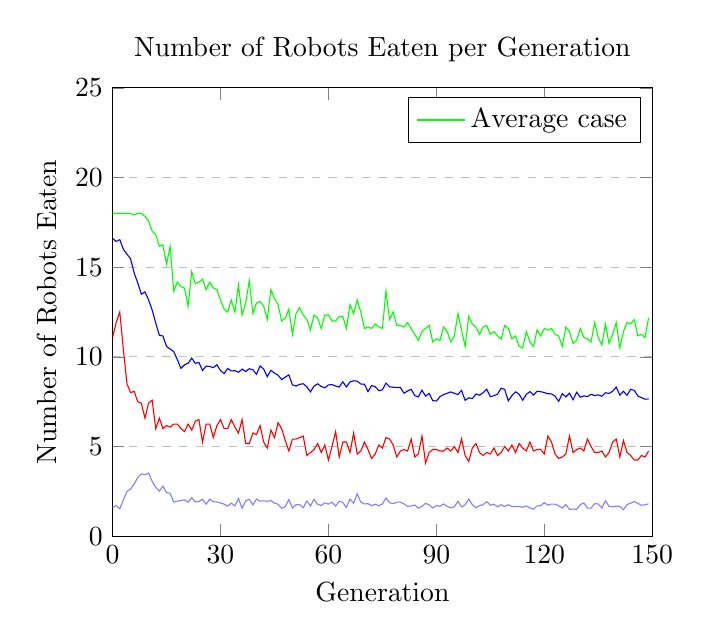
\begin{tikzpicture}
\begin{axis}[
	title={Number of Robots Eaten per Generation},
	xlabel={Generation},
	ylabel={Number of Robots Eaten},
	xmin=0, xmax=150,
	ymin=0, ymax=25,
	xtick={0.0,30.0,60.0,90.0,120.0,150.0},
	ytick={0.0,5.0,10.0,15.0,20.0,25.0},
	ymajorgrids=true,
	grid style=dashed,
]

\addplot[
	color=green,
	]
	coordinates {
	(0,18.0)(1,18.0)(2,18.0)(3,18.0)(4,18.0)(5,18.0)(6,17.916666666666668)(7,18.0)(8,18.0)(9,17.833333333333332)(10,17.583333333333332)(11,17.0)(12,16.833333333333336)(13,16.166666666666664)(14,16.25)(15,15.166666666666666)(16,16.166666666666668)(17,13.666666666666668)(18,14.166666666666666)(19,13.916666666666666)(20,13.833333333333332)(21,12.833333333333334)(22,14.750000000000002)(23,14.083333333333334)(24,14.166666666666668)(25,14.333333333333334)(26,13.75)(27,14.166666666666668)(28,13.833333333333334)(29,13.75)(30,13.166666666666666)(31,12.666666666666668)(32,12.5)(33,13.166666666666666)(34,12.5)(35,14.000000000000002)(36,12.333333333333334)(37,13.0)(38,14.25)(39,12.416666666666666)(40,13.0)(41,13.083333333333334)(42,12.833333333333334)(43,12.083333333333334)(44,13.75)(45,13.25)(46,12.916666666666666)(47,12.0)(48,12.166666666666666)(49,12.666666666666666)(50,11.25)(51,12.416666666666666)(52,12.750000000000002)(53,12.333333333333334)(54,12.083333333333334)(55,11.5)(56,12.333333333333334)(57,12.166666666666666)(58,11.583333333333334)(59,12.333333333333334)(60,12.333333333333334)(61,12.0)(62,12.000000000000002)(63,12.250000000000002)(64,12.25)(65,11.583333333333334)(66,12.916666666666666)(67,12.416666666666666)(68,13.166666666666666)(69,12.5)(70,11.583333333333334)(71,11.666666666666666)(72,11.583333333333332)(73,11.833333333333334)(74,11.666666666666666)(75,11.583333333333334)(76,13.666666666666668)(77,12.083333333333334)(78,12.5)(79,11.75)(80,11.75)(81,11.666666666666666)(82,11.916666666666666)(83,11.583333333333332)(84,11.25)(85,10.916666666666668)(86,11.416666666666668)(87,11.583333333333332)(88,11.75)(89,10.833333333333334)(90,11.0)(91,10.916666666666666)(92,11.666666666666668)(93,11.416666666666666)(94,10.833333333333334)(95,11.166666666666666)(96,12.416666666666666)(97,11.5)(98,10.583333333333334)(99,12.25)(100,11.833333333333334)(101,11.666666666666666)(102,11.25)(103,11.666666666666666)(104,11.75)(105,11.249999999999998)(106,11.416666666666668)(107,11.166666666666666)(108,11.0)(109,11.750000000000002)(110,11.583333333333334)(111,11.0)(112,11.166666666666666)(113,10.583333333333334)(114,10.5)(115,11.416666666666666)(116,10.833333333333334)(117,10.583333333333332)(118,11.500000000000002)(119,11.166666666666668)(120,11.583333333333334)(121,11.500000000000002)(122,11.583333333333334)(123,11.25)(124,11.166666666666666)(125,10.583333333333334)(126,11.666666666666668)(127,11.416666666666666)(128,10.749999999999998)(129,10.916666666666668)(130,11.583333333333332)(131,11.083333333333334)(132,11.0)(133,10.833333333333332)(134,11.916666666666668)(135,11.083333333333334)(136,10.666666666666666)(137,11.833333333333334)(138,10.75)(139,11.250000000000002)(140,11.916666666666666)(141,10.5)(142,11.416666666666666)(143,11.916666666666666)(144,11.833333333333334)(145,12.083333333333334)(146,11.166666666666666)(147,11.250000000000002)(148,11.083333333333334)(149,12.166666666666668)
	};
\addplot[
	color=blue,
	]
	coordinates {
	(0,16.604166666666664)(1,16.4375)(2,16.538194444444443)(3,16.0)(4,15.729166666666668)(5,15.468750000000002)(6,14.677083333333334)(7,14.125)(8,13.493055555555555)(9,13.621527777777779)(10,13.180555555555557)(11,12.618055555555557)(12,11.88541666666667)(13,11.20486111111111)(14,11.163194444444445)(15,10.57986111111111)(16,10.440972222222221)(17,10.291666666666668)(18,9.84375)(19,9.36111111111111)(20,9.559027777777779)(21,9.64236111111111)(22,9.930555555555555)(23,9.63888888888889)(24,9.6875)(25,9.243055555555557)(26,9.479166666666668)(27,9.465277777777779)(28,9.402777777777777)(29,9.559027777777777)(30,9.23611111111111)(31,9.069444444444445)(32,9.354166666666668)(33,9.215277777777779)(34,9.23263888888889)(35,9.13888888888889)(36,9.315972222222223)(37,9.184027777777779)(38,9.336805555555557)(39,9.284722222222221)(40,9.027777777777779)(41,9.493055555555554)(42,9.322916666666666)(43,8.895833333333332)(44,9.25)(45,9.097222222222221)(46,8.98263888888889)(47,8.73263888888889)(48,8.868055555555555)(49,8.996527777777777)(50,8.4375)(51,8.371527777777779)(52,8.46875)(53,8.5)(54,8.32986111111111)(55,8.04861111111111)(56,8.368055555555557)(57,8.496527777777779)(58,8.350694444444446)(59,8.274305555555555)(60,8.4375)(61,8.45138888888889)(62,8.371527777777779)(63,8.319444444444445)(64,8.61111111111111)(65,8.319444444444445)(66,8.604166666666668)(67,8.666666666666668)(68,8.645833333333334)(69,8.48611111111111)(70,8.472222222222221)(71,8.065972222222223)(72,8.399305555555555)(73,8.336805555555554)(74,8.114583333333332)(75,8.163194444444446)(76,8.538194444444445)(77,8.329861111111112)(78,8.305555555555557)(79,8.288194444444445)(80,8.29513888888889)(81,7.975694444444444)(82,8.09375)(83,8.194444444444446)(84,7.840277777777778)(85,7.767361111111112)(86,8.14236111111111)(87,7.809027777777778)(88,7.961805555555556)(89,7.562500000000001)(90,7.5381944444444455)(91,7.777777777777779)(92,7.895833333333333)(93,7.96875)(94,8.04513888888889)(95,7.968749999999999)(96,7.895833333333335)(97,8.128472222222223)(98,7.5763888888888875)(99,7.715277777777779)(100,7.673611111111111)(101,7.927083333333333)(102,7.861111111111111)(103,8.0)(104,8.197916666666668)(105,7.781249999999999)(106,7.833333333333333)(107,7.920138888888889)(108,8.253472222222221)(109,8.184027777777779)(110,7.548611111111112)(111,7.840277777777779)(112,8.052083333333334)(113,7.920138888888889)(114,7.579861111111111)(115,7.90625)(116,8.0625)(117,7.868055555555555)(118,8.083333333333334)(119,8.055555555555555)(120,8.010416666666666)(121,7.944444444444444)(122,7.9375)(123,7.809027777777777)(124,7.517361111111111)(125,7.951388888888891)(126,7.767361111111111)(127,7.972222222222221)(128,7.611111111111111)(129,8.027777777777779)(130,7.75)(131,7.826388888888889)(132,7.784722222222222)(133,7.913194444444445)(134,7.840277777777778)(135,7.8819444444444455)(136,7.798611111111112)(137,8.0)(138,7.958333333333334)(139,8.07986111111111)(140,8.3125)(141,7.864583333333334)(142,8.083333333333334)(143,7.857638888888889)(144,8.190972222222221)(145,8.135416666666668)(146,7.819444444444445)(147,7.732638888888888)(148,7.638888888888888)(149,7.649305555555556)
	};
	\addlegendentry{Average case}
\addplot[
	color=red,
	]
	coordinates {
	(0,11.083333333333334)(1,11.916666666666666)(2,12.5)(3,10.416666666666666)(4,8.5)(5,8.0)(6,8.083333333333332)(7,7.5)(8,7.416666666666666)(9,6.583333333333333)(10,7.416666666666668)(11,7.583333333333333)(12,6.0)(13,6.583333333333333)(14,6.0)(15,6.166666666666666)(16,6.083333333333333)(17,6.250000000000001)(18,6.250000000000001)(19,6.0)(20,5.833333333333334)(21,6.25)(22,5.916666666666667)(23,6.416666666666667)(24,6.5)(25,5.249999999999999)(26,6.250000000000001)(27,6.25)(28,5.5)(29,6.166666666666667)(30,6.500000000000001)(31,6.0)(32,5.999999999999999)(33,6.5)(34,6.083333333333334)(35,5.750000000000001)(36,6.5)(37,5.166666666666667)(38,5.166666666666666)(39,5.75)(40,5.666666666666667)(41,6.166666666666667)(42,5.25)(43,4.916666666666667)(44,5.916666666666667)(45,5.5)(46,6.333333333333334)(47,6.0)(48,5.333333333333333)(49,4.75)(50,5.416666666666667)(51,5.416666666666667)(52,5.5)(53,5.583333333333334)(54,4.5)(55,4.666666666666667)(56,4.833333333333333)(57,5.166666666666667)(58,4.666666666666667)(59,5.083333333333334)(60,4.25)(61,5.0)(62,5.833333333333334)(63,4.416666666666667)(64,5.25)(65,5.25)(66,4.666666666666667)(67,5.75)(68,4.583333333333333)(69,4.75)(70,5.250000000000001)(71,4.833333333333333)(72,4.333333333333333)(73,4.583333333333333)(74,5.083333333333333)(75,4.916666666666667)(76,5.5)(77,5.416666666666667)(78,5.083333333333333)(79,4.416666666666666)(80,4.75)(81,4.833333333333334)(82,4.75)(83,5.416666666666666)(84,4.416666666666667)(85,4.583333333333333)(86,5.583333333333334)(87,4.083333333333334)(88,4.666666666666666)(89,4.833333333333333)(90,4.833333333333334)(91,4.75)(92,4.75)(93,4.916666666666667)(94,4.75)(95,5.0)(96,4.666666666666666)(97,5.416666666666667)(98,4.5)(99,4.166666666666667)(100,4.916666666666667)(101,5.166666666666667)(102,4.666666666666667)(103,4.5)(104,4.666666666666667)(105,4.583333333333333)(106,4.916666666666667)(107,4.5)(108,4.666666666666667)(109,5.0)(110,4.75)(111,5.083333333333334)(112,4.666666666666667)(113,5.166666666666667)(114,4.916666666666666)(115,4.75)(116,5.25)(117,4.75)(118,4.833333333333333)(119,4.833333333333334)(120,4.583333333333333)(121,5.583333333333334)(122,5.25)(123,4.583333333333334)(124,4.333333333333333)(125,4.416666666666667)(126,4.583333333333333)(127,5.583333333333333)(128,4.666666666666667)(129,4.833333333333333)(130,4.916666666666666)(131,4.75)(132,5.416666666666667)(133,5.0)(134,4.666666666666667)(135,4.666666666666667)(136,4.75)(137,4.416666666666667)(138,4.666666666666667)(139,5.25)(140,5.416666666666667)(141,4.416666666666667)(142,5.333333333333333)(143,4.666666666666667)(144,4.5)(145,4.25)(146,4.25)(147,4.5)(148,4.416666666666667)(149,4.750000000000001)
	};
\addplot[
	color=blue!50,
	]
	coordinates {
	(0,1.6135628189321447)(1,1.7026949044554263)(2,1.5291905797757304)(3,2.025632238096803)(4,2.4912280515381684)(5,2.62450422996143)(6,2.9075554247373283)(7,3.269779059018078)(8,3.469457246017191)(9,3.4259631465127622)(10,3.520904998759863)(11,3.0568091836636753)(12,2.7286965077778187)(13,2.5050367716339386)(14,2.7868811997902627)(15,2.4286899117935743)(16,2.394493936735425)(17,1.902432205702461)(18,1.9554252837892947)(19,1.986622541145191)(20,2.023747601549805)(21,1.8960104140755112)(22,2.149467183460963)(23,1.9099497785901267)(24,1.9390235926933905)(25,2.057076550380303)(26,1.7838124480399062)(27,2.064839387475817)(28,1.9214142292224907)(29,1.9083006769569955)(30,1.8522945517696492)(31,1.7853420882445976)(32,1.6738899148549757)(33,1.8424649929408177)(34,1.6866420194516545)(35,2.092139627380162)(36,1.5556426111957142)(37,1.9711989322677241)(38,2.060946378774058)(39,1.747994490566172)(40,2.074756953311265)(41,1.9506052180687645)(42,1.9757035285735494)(43,1.9446054532177541)(44,1.9946107754920686)(45,1.8407752508102047)(46,1.7855575029428408)(47,1.5580167188982954)(48,1.6514828114744518)(49,2.0433505197817974)(50,1.5644294651713557)(51,1.7539706609190224)(52,1.7589804314518234)(53,1.5893022059670032)(54,1.965783328411519)(55,1.6915127657966957)(56,2.055634935058416)(57,1.7794492094324876)(58,1.7143412361708394)(59,1.8624627110307803)(60,1.790278568793217)(61,1.8950958275011192)(62,1.6836265087430493)(63,1.956697603144673)(64,1.880028369064952)(65,1.6040685585360883)(66,2.06947246185333)(67,1.8275824518511863)(68,2.3665468558358085)(69,1.900985316270165)(70,1.7967403731578835)(71,1.815961043075833)(72,1.7011998334085106)(73,1.7856749736892323)(74,1.6977915190697386)(75,1.7972645059064396)(76,2.1276524656893123)(77,1.8653656326546653)(78,1.8184207960408596)(79,1.8968929700639263)(80,1.8999946919687736)(81,1.798475378371157)(82,1.6686783698760659)(83,1.677330139789346)(84,1.7333290764308584)(85,1.5665310283865717)(86,1.6679108862995395)(87,1.8314244255358991)(88,1.7462520697984318)(89,1.5728759250902709)(90,1.710881726716985)(91,1.6664670992250499)(92,1.7988049412204024)(93,1.6645423396256416)(94,1.5781590426939909)(95,1.6403417655074377)(96,1.9419874376897766)(97,1.6349338528695097)(98,1.7435818935837624)(99,2.074029284617884)(100,1.7596251353598915)(101,1.5816552998082343)(102,1.7100559169416756)(103,1.7563481956372775)(104,1.9301918417259356)(105,1.7262480140446073)(106,1.7832159443613889)(107,1.637703522552553)(108,1.7569343739159362)(109,1.652079563648607)(110,1.75394267790958)(111,1.65671102974029)(112,1.6532759247788724)(113,1.653398645774141)(114,1.6144304303980501)(115,1.6868907839954936)(116,1.5777295443736665)(117,1.5034650286673994)(118,1.6911032563165835)(119,1.7010369146266267)(120,1.8745362801034413)(121,1.724055128881595)(122,1.7913102536457433)(123,1.7837861422723336)(124,1.7003904581061589)(125,1.565831438885306)(126,1.7610468815579396)(127,1.4954158715351333)(128,1.5130552316460117)(129,1.4937537312856826)(130,1.7549153991261395)(131,1.8562698904514678)(132,1.5691800731418324)(133,1.5653605781621032)(134,1.8119904597969572)(135,1.7980523281459233)(136,1.5677460720436147)(137,1.9753999591781781)(138,1.66799233375207)(139,1.6346176715988017)(140,1.6745676849866808)(141,1.6646644576599574)(142,1.47522496940006)(143,1.7645574261265964)(144,1.8381721537429572)(145,1.9280790101739624)(146,1.8329986055600598)(147,1.7189596764545994)(148,1.752398037108075)(149,1.8053866533060816)
	};
\end{axis}
\end{tikzpicture}
}
		\caption{Some sample caption}
		\label{fig:easy-robots-eaten}
	\end{subfigure}%
}
\\
\\
\\
	\makebox[\linewidth][c]{%
	\begin{subfigure}[b]{0.7\textwidth}
		\centering
		\resizebox{0.9\linewidth}{!}{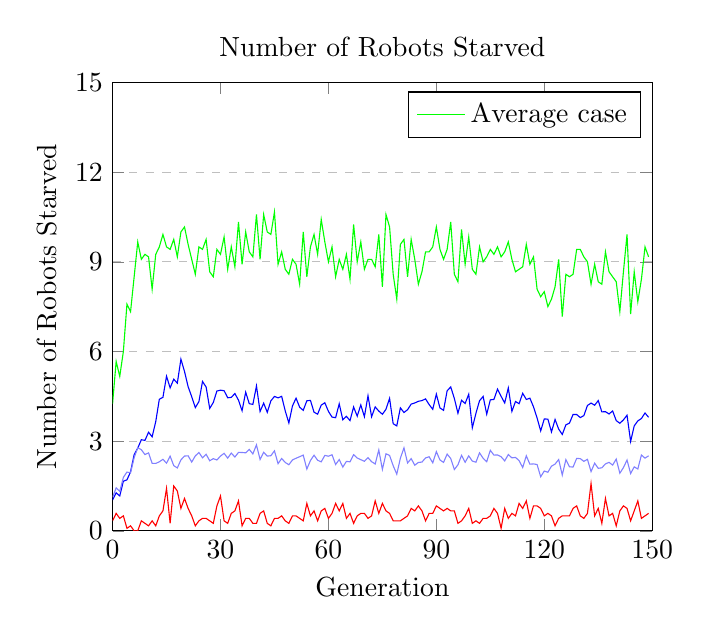
\begin{tikzpicture}
\begin{axis}[
	title={Number of Robots Starved},
	xlabel={Generation},
	ylabel={Number of Robots Starved},
	xmin=0, xmax=150,
	ymin=0, ymax=15,
	xtick={0.0,30.0,60.0,90.0,120.0,150.0},
	ytick={0.0,3.0,6.0,9.0,12.0,15.0},
	ymajorgrids=true,
	grid style=dashed,
]

\addplot[
	color=green,
	]
	coordinates {
	(0,4.25)(1,5.666666666666667)(2,5.166666666666666)(3,6.0)(4,7.583333333333333)(5,7.333333333333334)(6,8.5)(7,9.666666666666668)(8,9.083333333333334)(9,9.25)(10,9.166666666666666)(11,8.083333333333334)(12,9.25)(13,9.5)(14,9.916666666666666)(15,9.5)(16,9.416666666666666)(17,9.75)(18,9.166666666666668)(19,10.0)(20,10.166666666666666)(21,9.583333333333334)(22,9.083333333333332)(23,8.583333333333334)(24,9.5)(25,9.416666666666666)(26,9.75)(27,8.666666666666668)(28,8.5)(29,9.416666666666666)(30,9.250000000000002)(31,9.833333333333334)(32,8.75)(33,9.5)(34,8.833333333333332)(35,10.333333333333332)(36,8.916666666666666)(37,10.0)(38,9.333333333333334)(39,9.166666666666666)(40,10.583333333333334)(41,9.083333333333334)(42,10.583333333333334)(43,10.0)(44,9.916666666666666)(45,10.666666666666666)(46,8.916666666666668)(47,9.333333333333334)(48,8.75)(49,8.583333333333334)(50,9.083333333333332)(51,8.916666666666668)(52,8.25)(53,10.0)(54,8.5)(55,9.5)(56,9.916666666666668)(57,9.25)(58,10.416666666666666)(59,9.666666666666666)(60,9.0)(61,9.5)(62,8.5)(63,9.083333333333334)(64,8.75)(65,9.25)(66,8.416666666666668)(67,10.25)(68,9.0)(69,9.666666666666666)(70,8.75)(71,9.083333333333334)(72,9.083333333333334)(73,8.833333333333334)(74,9.916666666666666)(75,8.166666666666668)(76,10.583333333333332)(77,10.166666666666668)(78,8.583333333333334)(79,7.749999999999999)(80,9.583333333333334)(81,9.75)(82,8.5)(83,9.75)(84,9.083333333333332)(85,8.25)(86,8.666666666666666)(87,9.333333333333334)(88,9.333333333333334)(89,9.5)(90,10.166666666666666)(91,9.416666666666668)(92,9.083333333333332)(93,9.416666666666668)(94,10.333333333333334)(95,8.583333333333332)(96,8.333333333333332)(97,10.083333333333334)(98,8.916666666666668)(99,9.833333333333334)(100,8.75)(101,8.583333333333334)(102,9.5)(103,9.000000000000002)(104,9.166666666666666)(105,9.416666666666666)(106,9.25)(107,9.5)(108,9.166666666666668)(109,9.333333333333332)(110,9.666666666666666)(111,9.083333333333334)(112,8.666666666666668)(113,8.75)(114,8.833333333333332)(115,9.583333333333332)(116,8.916666666666666)(117,9.166666666666668)(118,8.083333333333334)(119,7.833333333333332)(120,8.0)(121,7.5)(122,7.75)(123,8.166666666666668)(124,9.083333333333334)(125,7.166666666666667)(126,8.583333333333334)(127,8.5)(128,8.583333333333334)(129,9.416666666666666)(130,9.416666666666666)(131,9.166666666666666)(132,9.0)(133,8.25)(134,8.916666666666666)(135,8.333333333333334)(136,8.25)(137,9.333333333333332)(138,8.666666666666666)(139,8.5)(140,8.333333333333334)(141,7.333333333333334)(142,8.666666666666666)(143,9.916666666666666)(144,7.25)(145,8.666666666666668)(146,7.666666666666666)(147,8.416666666666666)(148,9.5)(149,9.166666666666666)
	};
\addplot[
	color=blue,
	]
	coordinates {
	(0,1.0277777777777777)(1,1.2708333333333335)(2,1.1666666666666665)(3,1.6597222222222223)(4,1.7048611111111114)(5,1.972222222222222)(6,2.548611111111111)(7,2.767361111111111)(8,3.048611111111111)(9,3.0243055555555554)(10,3.298611111111111)(11,3.1458333333333335)(12,3.6527777777777777)(13,4.402777777777779)(14,4.465277777777778)(15,5.173611111111111)(16,4.78125)(17,5.072916666666667)(18,4.940972222222222)(19,5.7430555555555545)(20,5.3298611111111125)(21,4.822916666666667)(22,4.486111111111111)(23,4.121527777777778)(24,4.322916666666667)(25,4.996527777777779)(26,4.8125)(27,4.09375)(28,4.295138888888888)(29,4.677083333333333)(30,4.704861111111111)(31,4.6875)(32,4.451388888888889)(33,4.465277777777778)(34,4.59375)(35,4.371527777777778)(36,4.017361111111111)(37,4.638888888888888)(38,4.253472222222223)(39,4.229166666666666)(40,4.847222222222222)(41,3.993055555555556)(42,4.270833333333334)(43,3.9652777777777777)(44,4.347222222222222)(45,4.496527777777778)(46,4.447916666666668)(47,4.5)(48,4.010416666666667)(49,3.6076388888888893)(50,4.177083333333333)(51,4.4375)(52,4.135416666666667)(53,4.03125)(54,4.350694444444445)(55,4.364583333333333)(56,3.968749999999999)(57,3.9027777777777777)(58,4.204861111111111)(59,4.284722222222222)(60,3.9965277777777777)(61,3.8055555555555554)(62,3.7847222222222223)(63,4.25)(64,3.7152777777777786)(65,3.829861111111111)(66,3.6875)(67,4.142361111111112)(68,3.8368055555555554)(69,4.211805555555555)(70,3.8194444444444446)(71,4.517361111111112)(72,3.8159722222222223)(73,4.145833333333334)(74,4.006944444444445)(75,3.8993055555555554)(76,4.065972222222223)(77,4.427083333333333)(78,3.583333333333333)(79,3.510416666666666)(80,4.114583333333334)(81,3.958333333333334)(82,4.052083333333334)(83,4.239583333333333)(84,4.277777777777777)(85,4.333333333333334)(86,4.357638888888888)(87,4.413194444444444)(88,4.222222222222223)(89,4.065972222222222)(90,4.572916666666667)(91,4.111111111111111)(92,4.03125)(93,4.6875)(94,4.8125)(95,4.430555555555555)(96,3.9340277777777777)(97,4.368055555555555)(98,4.260416666666667)(99,4.569444444444445)(100,3.4479166666666665)(101,3.9305555555555554)(102,4.350694444444445)(103,4.496527777777778)(104,3.9027777777777777)(105,4.381944444444445)(106,4.395833333333333)(107,4.739583333333334)(108,4.5)(109,4.277777777777778)(110,4.78125)(111,3.9965277777777777)(112,4.326388888888888)(113,4.253472222222221)(114,4.6006944444444455)(115,4.395833333333333)(116,4.437499999999999)(117,4.149305555555555)(118,3.7743055555555554)(119,3.34375)(120,3.7430555555555562)(121,3.7361111111111107)(122,3.309027777777778)(123,3.7256944444444446)(124,3.4027777777777777)(125,3.2222222222222223)(126,3.5451388888888893)(127,3.604166666666667)(128,3.8923611111111116)(129,3.8923611111111107)(130,3.7881944444444438)(131,3.854166666666667)(132,4.194444444444444)(133,4.274305555555555)(134,4.201388888888889)(135,4.357638888888889)(136,3.9791666666666665)(137,3.9861111111111116)(138,3.9097222222222228)(139,4.010416666666667)(140,3.6875)(141,3.5972222222222223)(142,3.7118055555555554)(143,3.8680555555555562)(144,2.9895833333333335)(145,3.5104166666666665)(146,3.677083333333333)(147,3.756944444444445)(148,3.9409722222222223)(149,3.7986111111111107)
	};
	\addlegendentry{Average case}
\addplot[
	color=red,
	]
	coordinates {
	(0,0.3333333333333333)(1,0.5833333333333333)(2,0.41666666666666663)(3,0.5)(4,0.08333333333333333)(5,0.16666666666666666)(6,0.0)(7,0.0)(8,0.3333333333333333)(9,0.25)(10,0.16666666666666666)(11,0.3333333333333333)(12,0.16666666666666666)(13,0.5)(14,0.6666666666666666)(15,1.4166666666666667)(16,0.25)(17,1.5)(18,1.3333333333333333)(19,0.75)(20,1.0833333333333333)(21,0.75)(22,0.5)(23,0.16666666666666666)(24,0.3333333333333333)(25,0.41666666666666663)(26,0.41666666666666663)(27,0.3333333333333333)(28,0.25)(29,0.8333333333333333)(30,1.1666666666666665)(31,0.3333333333333333)(32,0.25)(33,0.5833333333333334)(34,0.6666666666666666)(35,1.0)(36,0.16666666666666666)(37,0.41666666666666663)(38,0.41666666666666663)(39,0.25)(40,0.25)(41,0.5833333333333333)(42,0.6666666666666666)(43,0.25)(44,0.16666666666666666)(45,0.4166666666666667)(46,0.41666666666666663)(47,0.5)(48,0.3333333333333333)(49,0.25)(50,0.5)(51,0.5)(52,0.41666666666666663)(53,0.3333333333333333)(54,0.9166666666666667)(55,0.5)(56,0.6666666666666667)(57,0.3333333333333333)(58,0.6666666666666666)(59,0.75)(60,0.41666666666666663)(61,0.5833333333333334)(62,0.9166666666666666)(63,0.6666666666666666)(64,0.9166666666666667)(65,0.4166666666666667)(66,0.5833333333333334)(67,0.25)(68,0.49999999999999994)(69,0.5833333333333333)(70,0.5833333333333334)(71,0.4166666666666667)(72,0.5)(73,0.9999999999999999)(74,0.5833333333333333)(75,0.9166666666666666)(76,0.6666666666666666)(77,0.5833333333333333)(78,0.3333333333333333)(79,0.3333333333333333)(80,0.3333333333333333)(81,0.41666666666666663)(82,0.5)(83,0.75)(84,0.6666666666666667)(85,0.8333333333333334)(86,0.6666666666666666)(87,0.3333333333333333)(88,0.5833333333333334)(89,0.5833333333333334)(90,0.8333333333333333)(91,0.7499999999999999)(92,0.6666666666666667)(93,0.75)(94,0.6666666666666667)(95,0.6666666666666666)(96,0.25)(97,0.3333333333333333)(98,0.5)(99,0.7499999999999999)(100,0.25)(101,0.3333333333333333)(102,0.25)(103,0.41666666666666663)(104,0.41666666666666663)(105,0.5)(106,0.75)(107,0.5833333333333334)(108,0.08333333333333333)(109,0.75)(110,0.41666666666666663)(111,0.5833333333333334)(112,0.5)(113,0.9166666666666667)(114,0.75)(115,1.0)(116,0.41666666666666663)(117,0.8333333333333334)(118,0.8333333333333334)(119,0.75)(120,0.5)(121,0.5833333333333334)(122,0.5)(123,0.16666666666666666)(124,0.41666666666666663)(125,0.49999999999999994)(126,0.5)(127,0.5)(128,0.75)(129,0.8333333333333333)(130,0.5)(131,0.41666666666666663)(132,0.5833333333333334)(133,1.5833333333333335)(134,0.49999999999999994)(135,0.75)(136,0.25)(137,1.0833333333333335)(138,0.5)(139,0.5833333333333333)(140,0.16666666666666666)(141,0.6666666666666666)(142,0.8333333333333333)(143,0.75)(144,0.3333333333333333)(145,0.6666666666666667)(146,1.0)(147,0.41666666666666663)(148,0.5)(149,0.5833333333333333)
	};
\addplot[
	color=blue!50,
	]
	coordinates {
	(0,1.1186666502498601)(1,1.4375000281055272)(2,1.320256431806563)(3,1.7870304672552086)(4,1.9654411846815782)(5,1.9419915165254884)(6,2.4479457948121075)(7,2.781315029033354)(8,2.713530073076882)(9,2.551238753438123)(10,2.607395241535058)(11,2.257697655051219)(12,2.253931931510418)(13,2.309557324956686)(14,2.391696603082267)(15,2.2631751898076597)(16,2.498347125363523)(17,2.1825619023483354)(18,2.1028863106782243)(19,2.3735772370777157)(20,2.5013713788384355)(21,2.509444055691578)(22,2.301083617664844)(23,2.506101750564102)(24,2.6204625402824537)(25,2.440743357213416)(26,2.561956738396159)(27,2.343698177191451)(28,2.4142425127275455)(29,2.3697815008779006)(30,2.500033163552189)(31,2.592396363264087)(32,2.4318849211795213)(33,2.600305222671007)(34,2.4688052280941237)(35,2.623176764359093)(36,2.6206826304736435)(37,2.6094646507318897)(38,2.7212458758258644)(39,2.5727046396267905)(40,2.8740354295630994)(41,2.3864452614819776)(42,2.6269076390179604)(43,2.4995211196463214)(44,2.512866665238211)(45,2.675642777531086)(46,2.2459033362090337)(47,2.4203023084028925)(48,2.287165212360806)(49,2.2102034033580313)(50,2.3695422861647977)(51,2.4280926503868274)(52,2.478903280244368)(53,2.5330855888024755)(54,2.0661602149546443)(55,2.350242569127601)(56,2.529726743883363)(57,2.3601933211925727)(58,2.308152362065781)(59,2.522727699963753)(60,2.4966092772079946)(61,2.544165665831553)(62,2.2188219385425314)(63,2.384255998869686)(64,2.131187063976123)(65,2.32393712879922)(66,2.307899768125281)(67,2.547969480630482)(68,2.436268343257018)(69,2.3802803771988383)(70,2.3251723243980513)(71,2.446840390640039)(72,2.313396908020027)(73,2.236241721885899)(74,2.7057894710684933)(75,2.0547161995549343)(76,2.5769658736280268)(77,2.5216300639434825)(78,2.1786296995579244)(79,1.8952280631805452)(80,2.429532421185556)(81,2.775990527114234)(82,2.269397322781032)(83,2.4160987471755275)(84,2.1959942969624793)(85,2.2862952545337842)(86,2.3000649747710975)(87,2.4383082307380914)(88,2.4773551245255647)(89,2.2752085873645664)(90,2.6492588337715963)(91,2.370968878340796)(92,2.2889837385629974)(93,2.567067841497752)(94,2.419123104453126)(95,2.050274530126912)(96,2.2072516930677124)(97,2.525201583207052)(98,2.2928185231041356)(99,2.5073861399815307)(100,2.3321653392086827)(101,2.2956970317411645)(102,2.6081328889818747)(103,2.4273331740517143)(104,2.312476777866677)(105,2.692797808303963)(106,2.53362277012872)(107,2.5375176524853096)(108,2.477407765300521)(109,2.338988240037007)(110,2.551850432078369)(111,2.440549707904938)(112,2.4561041178520897)(113,2.347791599240385)(114,2.1165376042683044)(115,2.5094766287940002)(116,2.2295209679428716)(117,2.2387677542848374)(118,2.217521605648701)(119,1.8074825400744043)(120,2.0003977502874752)(121,1.9606163205809013)(122,2.1626137589712977)(123,2.232275436529961)(124,2.3853474010706623)(125,1.8648846905293088)(126,2.380023544213634)(127,2.1435507120229285)(128,2.1321115988511)(129,2.4230490947099637)(130,2.4153187624353105)(131,2.3240550266551976)(132,2.3916772249253437)(133,1.9816198102436333)(134,2.262212120374356)(135,2.0900830618361987)(136,2.108946026058061)(137,2.238990685944853)(138,2.2899165641283767)(139,2.199842851010125)(140,2.4013089670381156)(141,1.9272046174430169)(142,2.114063712358885)(143,2.368919817605562)(144,1.9169700836306869)(145,2.1392615650178213)(146,2.068924501883676)(147,2.5353426993523858)(148,2.431507181307391)(149,2.5106721580580587)
	};
\end{axis}
\end{tikzpicture}
}
		\caption{Some sample caption}
		\label{fig:easy-robots-starved}
	\end{subfigure}%
	\begin{subfigure}[b]{0.7\textwidth}
		\centering
		\resizebox{0.9\linewidth}{!}{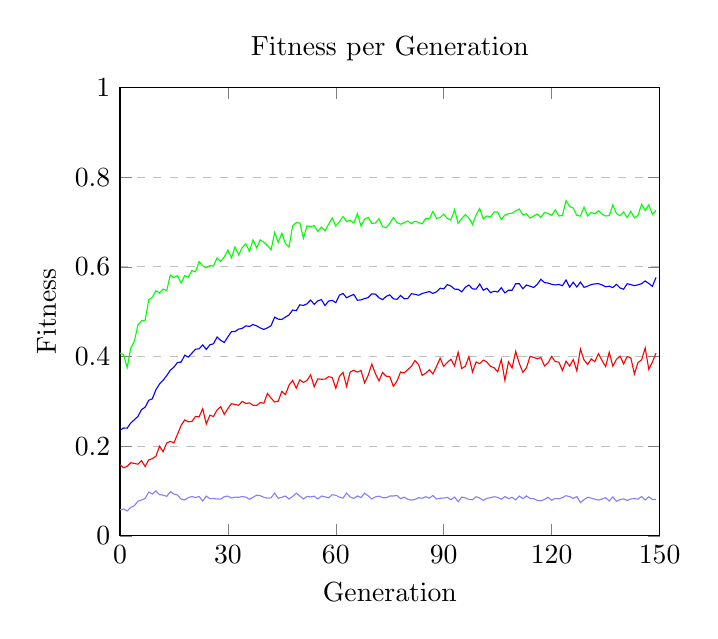
\begin{tikzpicture}
\begin{axis}[
	title={Fitness per Generation},
	xlabel={Generation},
	ylabel={Fitness},
	xmin=0, xmax=150,
	ymin=0, ymax=1,
	xtick={0.0,30.0,60.0,90.0,120.0,150.0},
	ytick={0.0,0.2,0.4,0.6000000000000001,0.8,1.0},
	ymajorgrids=true,
	grid style=dashed,
]

\addplot[
	color=green,
	]
	coordinates {
	(0,0.407433024691358)(1,0.40455246913580245)(2,0.375249537037037)(3,0.41873225308641987)(4,0.43406728395061733)(5,0.47047870370370376)(6,0.48000061728395077)(7,0.48074444444444436)(8,0.5266174382716049)(9,0.5326043209876542)(10,0.546644598765432)(11,0.5416791666666666)(12,0.550737037037037)(13,0.5472788580246913)(14,0.5818168209876543)(15,0.5762845679012346)(16,0.5803973765432099)(17,0.5637412037037037)(18,0.5807561728395062)(19,0.5770462962962962)(20,0.5918933641975308)(21,0.5890060185185186)(22,0.611758024691358)(23,0.6023779320987654)(24,0.597986574074074)(25,0.6028320987654322)(26,0.6018344135802469)(27,0.6198837962962963)(28,0.6122495370370372)(29,0.6220623456790124)(30,0.6373035493827159)(31,0.6203790123456789)(32,0.6443311728395062)(33,0.6266847222222223)(34,0.6429742283950617)(35,0.6516114197530866)(36,0.6346967592592594)(37,0.6601297839506174)(38,0.6424608024691357)(39,0.6603320987654321)(40,0.6550021604938272)(41,0.6473228395061729)(42,0.6378552469135802)(43,0.6765921296296297)(44,0.6545077160493827)(45,0.67522762345679)(46,0.6522231481481482)(47,0.6441180555555557)(48,0.6918532407407407)(49,0.6986695987654321)(50,0.6978850308641976)(51,0.6640128086419752)(52,0.6916970679012346)(53,0.6898421296296298)(54,0.6921731481481481)(55,0.6790364197530865)(56,0.6888367283950617)(57,0.6804623456790124)(58,0.6950320987654318)(59,0.7090398148148146)(60,0.6910038580246913)(61,0.7005773148148147)(62,0.7123285493827161)(63,0.701445987654321)(64,0.7039131172839507)(65,0.6975145061728395)(66,0.7190006172839506)(67,0.6912452160493827)(68,0.7063524691358025)(69,0.7106902777777777)(70,0.696969598765432)(71,0.6977742283950615)(72,0.7074362654320988)(73,0.6898623456790122)(74,0.6872458333333334)(75,0.6969765432098767)(76,0.7099206790123456)(77,0.699322685185185)(78,0.6952020061728394)(79,0.6986459876543211)(80,0.7024952160493828)(81,0.6961916666666669)(82,0.7019111111111112)(83,0.6990598765432098)(84,0.695925925925926)(85,0.7083817901234568)(86,0.7070557098765433)(87,0.7236819444444443)(88,0.7083805555555556)(89,0.7099149691358025)(90,0.7174049382716048)(91,0.7082470679012347)(92,0.7043149691358025)(93,0.7279672839506172)(94,0.6972297839506173)(95,0.7076268518518519)(96,0.7167833333333333)(97,0.7092716049382716)(98,0.6942013888888888)(99,0.7159430555555555)(100,0.7302199074074074)(101,0.7070033950617285)(102,0.7135929012345678)(103,0.7119015432098765)(104,0.7224578703703707)(105,0.7223239197530865)(106,0.7057788580246914)(107,0.7157495370370369)(108,0.7186895061728394)(109,0.7197694444444445)(110,0.7249671296296297)(111,0.7290618827160494)(112,0.7162617283950617)(113,0.7185904320987652)(114,0.7088546296296298)(115,0.7133479938271603)(116,0.71792237654321)(117,0.7102621913580247)(118,0.7212990740740741)(119,0.7193080246913581)(120,0.7151873456790123)(121,0.7271918209876542)(122,0.7135947530864198)(123,0.7149155864197531)(124,0.748066975308642)(125,0.73450987654321)(126,0.7312785493827161)(127,0.7150501543209877)(128,0.7132081790123458)(129,0.7334890432098767)(130,0.7137737654320988)(131,0.7214353395061728)(132,0.7183952160493826)(133,0.7253006172839508)(134,0.7177473765432097)(135,0.7134174382716051)(136,0.7144007716049384)(137,0.7385118827160495)(138,0.7191226851851853)(139,0.7142382716049382)(140,0.7225233024691359)(141,0.7100907407407406)(142,0.7240393518518519)(143,0.7093845679012346)(144,0.7148962962962964)(145,0.7397091049382715)(146,0.7257822530864197)(147,0.738746450617284)(148,0.7170873456790123)(149,0.7262729938271605)
	};
\addplot[
	color=blue,
	]
	coordinates {
	(0,0.23568551311728395)(1,0.24068541666666662)(2,0.24022112911522633)(3,0.25169717721193413)(4,0.2590899241255144)(5,0.2664853266460906)(6,0.28171860210905353)(7,0.2870059606481481)(8,0.3024511638374485)(9,0.30586267361111114)(10,0.3260418595679012)(11,0.338852070473251)(12,0.3473097029320988)(13,0.3574480195473251)(14,0.369612879372428)(15,0.3764822852366255)(16,0.38693112139917696)(17,0.38745133744855964)(18,0.40305448173868313)(19,0.39877369470164614)(20,0.40770316358024694)(21,0.41631231352880665)(22,0.417209921553498)(23,0.42592258873456784)(24,0.41594365997942395)(25,0.4262058513374486)(26,0.4285938078703704)(27,0.4435030671296296)(28,0.43614852752057603)(29,0.43139828960905346)(30,0.44385616640946496)(31,0.4555685635288066)(32,0.4559813914609053)(33,0.46119753086419757)(34,0.4630295910493827)(35,0.46848685699588477)(36,0.4671781121399177)(37,0.47134870113168725)(38,0.468452912808642)(39,0.4638823173868312)(40,0.4604523083847737)(41,0.46414776234567895)(42,0.46880528549382716)(43,0.48797928240740746)(44,0.4834216949588477)(45,0.48267862654320975)(46,0.48814235468107003)(47,0.4928079539609053)(48,0.5038436342592593)(49,0.5023217271090534)(50,0.5154713927469136)(51,0.5140101594650206)(52,0.5177034850823046)(53,0.5259832626028808)(54,0.5164022505144032)(55,0.5241722543724279)(56,0.5268482574588478)(57,0.5139078125000001)(58,0.5237850180041153)(59,0.5252607960390946)(60,0.5201704475308643)(61,0.5369881301440329)(62,0.5407399627057614)(63,0.5311644547325103)(64,0.5352260480967079)(65,0.5385806520061728)(66,0.5256074974279835)(67,0.5264563593106996)(68,0.5292461162551441)(69,0.5315578639403292)(70,0.5397327803497942)(71,0.5393159079218106)(72,0.5311407664609054)(73,0.5270274562757201)(74,0.5341304333847736)(75,0.537654140946502)(76,0.5289976466049382)(77,0.527455028292181)(78,0.5364096000514403)(79,0.5288648469650206)(80,0.5294152263374485)(81,0.5400965342078189)(82,0.5389623906893004)(83,0.5367551826131688)(84,0.5407509773662552)(85,0.5428390753600824)(86,0.5450959683641975)(87,0.54066875)(88,0.5444795717592592)(89,0.5525789030349794)(90,0.5508464441872428)(91,0.560527700617284)(92,0.5573773019547326)(93,0.5503285686728394)(94,0.5500769483024691)(95,0.5443369277263375)(96,0.5545731738683127)(97,0.5596265110596708)(98,0.5508877379115227)(99,0.5503951324588477)(100,0.5618264081790124)(101,0.5478969585905349)(102,0.5523157793209877)(103,0.5425106867283951)(104,0.5456846900720165)(105,0.543947633744856)(106,0.5536538966049382)(107,0.5419271219135802)(108,0.5479063657407407)(109,0.5477672260802469)(110,0.5625017554012345)(111,0.5624469071502058)(112,0.551313007973251)(113,0.5595609117798354)(114,0.5569121849279837)(115,0.5540847350823045)(116,0.5610753986625515)(117,0.572394045781893)(118,0.5649596129115226)(119,0.5639924382716048)(120,0.5611585390946502)(121,0.5596785236625514)(122,0.5608497620884774)(123,0.5581145640432099)(124,0.5709340534979425)(125,0.5549676826131686)(126,0.565735558127572)(127,0.5551598251028808)(128,0.5659945344650205)(129,0.5544160365226337)(130,0.5571219585905349)(131,0.5605994277263375)(132,0.5621280221193415)(133,0.5626246592078189)(134,0.5596513052983539)(135,0.555631880144033)(136,0.5569620177469135)(137,0.5538821180555557)(138,0.5610741190843622)(139,0.5530615162037038)(140,0.5501980259773662)(141,0.5625325360082304)(142,0.5604201903292181)(143,0.5582116576646091)(144,0.56005295781893)(145,0.5625418724279836)(146,0.568676517489712)(147,0.5630099408436213)(148,0.5567143840020575)(149,0.5763791538065843)
	};
\addplot[
	color=red,
	]
	coordinates {
	(0,0.15883472222222217)(1,0.15176620370370367)(2,0.15516774691358023)(3,0.16314398148148151)(4,0.16171574074074072)(5,0.1599047839506173)(6,0.167703549382716)(7,0.15460324074074072)(8,0.16965000000000008)(9,0.17227453703703707)(10,0.177687962962963)(11,0.20008703703703706)(12,0.1878003086419753)(13,0.20714043209876548)(14,0.21085910493827156)(15,0.2075063271604939)(16,0.2266248456790123)(17,0.2463229938271605)(18,0.2588023148148148)(19,0.25445648148148137)(20,0.2553297839506173)(21,0.2663185185185184)(22,0.26556466049382715)(23,0.28364907407407414)(24,0.24956651234567898)(25,0.26917608024691353)(26,0.266428086419753)(27,0.28083302469135807)(28,0.28820246913580233)(29,0.27107098765432097)(30,0.2839445987654321)(31,0.29507330246913577)(32,0.2930942901234568)(33,0.29139274691358025)(34,0.29994027777777776)(35,0.2953341049382716)(36,0.2966895061728395)(37,0.2912694444444444)(38,0.29084413580246915)(39,0.2974516975308642)(40,0.2958439814814814)(41,0.3177274691358025)(42,0.3072799382716051)(43,0.29868595679012344)(44,0.3005936728395062)(45,0.32242330246913586)(46,0.31510216049382717)(47,0.3362362654320988)(48,0.3466668209876543)(49,0.3295989197530865)(50,0.34805848765432096)(51,0.3424456790123457)(52,0.3466425925925927)(53,0.3592333333333333)(54,0.3325387345679012)(55,0.350087962962963)(56,0.3494266975308642)(57,0.3496253086419754)(58,0.35512654320987663)(59,0.3532475308641975)(60,0.3291945987654321)(61,0.3556766975308642)(62,0.3647975308641975)(63,0.333413425925926)(64,0.3656543209876543)(65,0.36919722222222223)(66,0.36540277777777774)(67,0.36901836419753076)(68,0.3412558641975309)(69,0.358175)(70,0.38318410493827154)(71,0.36207978395061735)(72,0.3456663580246913)(73,0.36432052469135806)(74,0.3562577160493827)(75,0.3551270061728395)(76,0.3336668209876544)(77,0.3450722222222221)(78,0.3654473765432099)(79,0.3635175925925926)(80,0.37078194444444446)(81,0.37806450617283943)(82,0.3910618827160493)(83,0.3824270061728395)(84,0.3579887345679014)(85,0.36289537037037034)(86,0.37047361111111116)(87,0.3612682098765431)(88,0.3780024691358025)(89,0.3961788580246913)(90,0.3779543209876544)(91,0.3867915123456791)(92,0.39410756172839495)(93,0.3790243827160495)(94,0.40976280864197534)(95,0.37320493827160484)(96,0.3783072530864198)(97,0.39986527777777775)(98,0.36572175925925915)(99,0.3879128086419752)(100,0.38413996913580256)(101,0.3921442901234568)(102,0.3878348765432098)(103,0.37821327160493823)(104,0.375004475308642)(105,0.366233024691358)(106,0.39331589506172837)(107,0.3468256172839506)(108,0.38828024691358026)(109,0.3746120370370371)(110,0.41167592592592595)(111,0.3846569444444444)(112,0.3648992283950617)(113,0.37512561728395066)(114,0.40050709876543217)(115,0.39813533950617286)(116,0.395041975308642)(117,0.3979228395061729)(118,0.37900709876543215)(119,0.3858986111111111)(120,0.40031790123456784)(121,0.3887069444444445)(122,0.3875763888888889)(123,0.36889583333333326)(124,0.3897364197530865)(125,0.37861111111111106)(126,0.3932961419753086)(127,0.3680199074074074)(128,0.4166959876543211)(129,0.3925061728395062)(130,0.3821908950617284)(131,0.39473148148148146)(132,0.38862083333333336)(133,0.4065702160493827)(134,0.3912300925925926)(135,0.3778217592592593)(136,0.4094202160493827)(137,0.3787717592592592)(138,0.3935929012345679)(139,0.4009652777777778)(140,0.38372129629629625)(141,0.40015725308641975)(142,0.39741929012345684)(143,0.36125802469135804)(144,0.3865432098765432)(145,0.3927938271604939)(146,0.41904459876543215)(147,0.37173317901234565)(148,0.3878891975308642)(149,0.4075714506172837)
	};
\addplot[
	color=blue!50,
	]
	coordinates {
	(0,0.058067186222303106)(1,0.05996962797552661)(2,0.055681990069950865)(3,0.06365291246859922)(4,0.06739382938509873)(5,0.07727518098752426)(6,0.079975080800059)(7,0.08365395212151348)(8,0.09767568767400732)(9,0.09359169003459027)(10,0.10028282642760386)(11,0.09195066418334417)(12,0.091014271388179)(13,0.08812308403579668)(14,0.09877289301055084)(15,0.09312541052798094)(16,0.09110473531942649)(17,0.08220092810608055)(18,0.08024209303710439)(19,0.0852989726920931)(20,0.08782583881748733)(21,0.08551136548662577)(22,0.08797029744155102)(23,0.07786202881228706)(24,0.08878824997677871)(25,0.08297547336566403)(26,0.08312604349707908)(27,0.08240536527181751)(28,0.08184094412059445)(29,0.08750535663556205)(30,0.08881841089807847)(31,0.0842701094167932)(32,0.08643562196348278)(33,0.08601208325004679)(34,0.08779408586634896)(35,0.08630315245409911)(36,0.08170972753578487)(37,0.08616308270139653)(38,0.0908901818900557)(39,0.08954975416446431)(40,0.08599894937034291)(41,0.08407768855535636)(42,0.08489615126348404)(43,0.09566199151941758)(44,0.08373056469044027)(45,0.08621788272733293)(46,0.08888885328832011)(47,0.08219180441536723)(48,0.08791580877392685)(49,0.09538713847842832)(50,0.0889370168706928)(51,0.08232162088566765)(52,0.08803664199070756)(53,0.0869451660555425)(54,0.08847666211756038)(55,0.08220717164220244)(56,0.08888597036621927)(57,0.0871425344527037)(58,0.08478240724768603)(59,0.0917152729287038)(60,0.09058301406799256)(61,0.08657430977690012)(62,0.08421695393666703)(63,0.09544644303835792)(64,0.08662144188339493)(65,0.08377620320150105)(66,0.08910338104282234)(67,0.08546466280854463)(68,0.09525637603289004)(69,0.08925946104960764)(70,0.08227119621187812)(71,0.08701379004628076)(72,0.08879454111930533)(73,0.08523872293370388)(74,0.08502240785897544)(75,0.08888168287751103)(76,0.08895684897065734)(77,0.0902485634654589)(78,0.08299321273788866)(79,0.0864775429755222)(80,0.08176144862485929)(81,0.07969689953953446)(82,0.08125523432036785)(83,0.08519378217309458)(84,0.08396116739597749)(85,0.08738936667831973)(86,0.0841783803246686)(87,0.09015048368691062)(88,0.08209189037413793)(89,0.08385707298207871)(90,0.08443464311943087)(91,0.085934928723441)(92,0.08059005231967695)(93,0.08672279877985603)(94,0.07633314961416324)(95,0.08655260025818795)(96,0.08487770271393649)(97,0.08105107867417133)(98,0.08066156877131667)(99,0.08737925317406545)(100,0.08436292178037316)(101,0.07914965139682562)(102,0.0838498186215269)(103,0.08502159834272127)(104,0.08735914894826724)(105,0.08596918438560495)(106,0.08168627693371408)(107,0.08766942656926588)(108,0.08298641055146984)(109,0.08603702534202752)(110,0.08038927658863951)(111,0.08898165909820657)(112,0.08291681662587534)(113,0.08919837327941246)(114,0.08344328429412487)(115,0.08297072401885405)(116,0.07915302497020739)(117,0.07811468247842442)(118,0.08124012640878209)(119,0.0861257686891845)(120,0.07927052170022521)(121,0.08357419638105776)(122,0.08265510724739608)(123,0.08529262449060622)(124,0.08976275178684359)(125,0.08750371219627105)(126,0.08350910193654089)(127,0.08790603945267966)(128,0.07416380710602953)(129,0.08088440398844952)(130,0.08612732589124428)(131,0.08416851934515088)(132,0.08201012771274403)(133,0.07982825130219404)(134,0.08225798998460179)(135,0.08522679990918171)(136,0.07782370444273558)(137,0.08696392309713072)(138,0.07713701816036178)(139,0.08064551018643046)(140,0.08258220097718316)(141,0.07916870134666855)(142,0.0823639145436908)(143,0.08305249430792266)(144,0.0822059423535918)(145,0.08760246354798056)(146,0.08003351171939858)(147,0.0871459975764063)(148,0.08110498208518849)(149,0.08085451774071063)
	};
\end{axis}
\end{tikzpicture}
}
		\caption{Some sample caption}
		\label{fig:easy-fitness}
	\end{subfigure}%
	
	
}
\caption{Figure shows results from a simulation in the easy environment (p.1)}
\end{figure}

\newpage
\vspace*{-2.0cm}
\textbf{\Huge Results -  Easy environment (2) }
\vspace{1.5cm}
\begin{tikzpicture}[remember picture,overlay]
   \node[anchor=south east,inner sep=20pt] at (current page.south east)
              {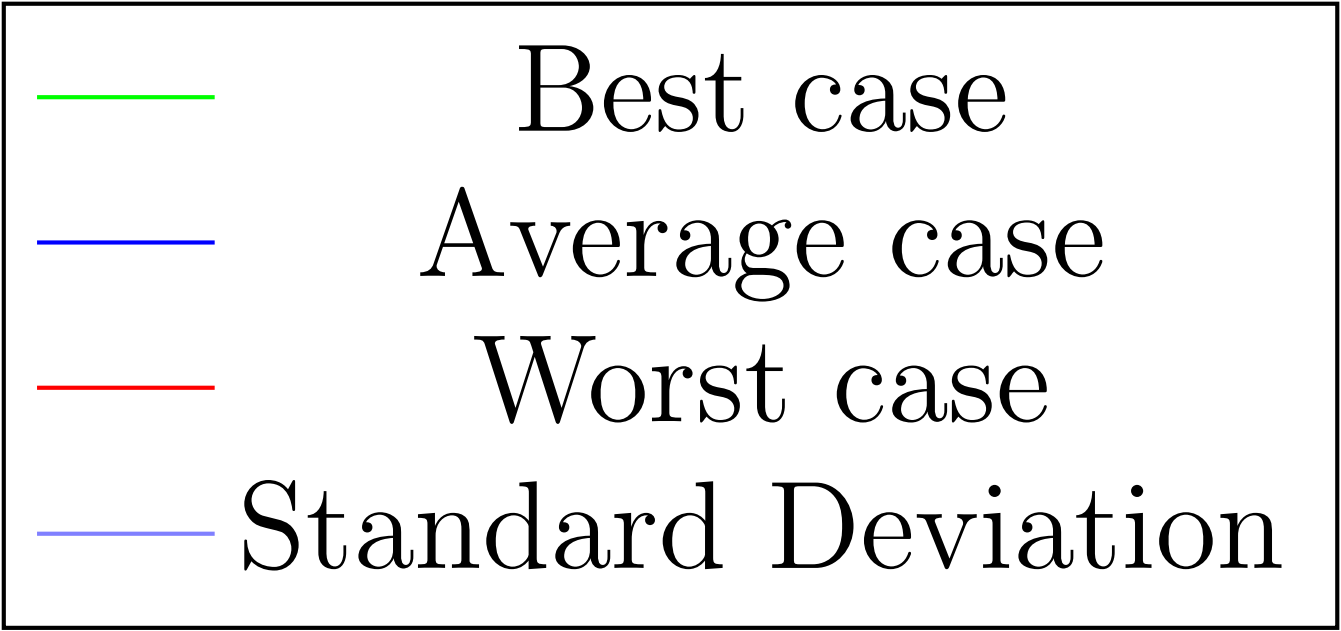
\includegraphics[scale=0.1]{chapters/res/generated_graph_legend.png}};
\end{tikzpicture}

\begin{figure}[H]
\vspace*{-1cm}
	\makebox[\linewidth][c]{%
	\begin{subfigure}[b]{0.7\textwidth}
		\centering
		\resizebox{0.9\linewidth}{!}{
        \begin{filecontents}{coord-easy-out.dat}
             x  y  r 
	 30 3 0.400000 
	 30 2 2.800000 
	 30 4 0.066667 
	 60 3 0.533333 
	 60 2 3.350000 
	 60 5 0.016667 
	 60 4 0.100000 
	 90 3 0.500000 
	 90 2 3.566667 
	 90 5 0.016667 
	 90 4 0.166667 
	 90 7 0.016667 
	 120 3 0.600000 
	 120 2 3.550000 
	 120 5 0.016667 
	 120 4 0.083333 
	 149 3 0.483333 
	 149 2 3.566667 
	 149 5 0.016667 
	 149 4 0.183333 
	 149 6 0.033333 

        \end{filecontents}
        
        \begin{tikzpicture}
        \begin{axis}[% scatter/use mapped color={draw=black,fill=mapped color},
        xmin=0, xmax=170,
        ymin=1, ymax=9,
        xtick={0.0,30.0,60.0,90.0,120.0,150.0},
        ytick={0.0,1.0,2.0,3.0,4.0,5.0, 6.0, 7.0, 8.0},]
        \addplot[scatter,scatter src=explicit, mark=*,only marks,
        % we use ’point meta’ as color data...
        point meta=\thisrow{y},
        % ... therefore, we can’t use it as argument for nodes near coords
        % ... which requires to define a visualization dependency:
        visualization depends on={value \thisrow{r} \as \r},
        scatter/@pre marker code/.append style=
        {/tikz/mark size=\r*3}
        ]
        table [x=x, y=y]
        {coord-easy-out.dat};
        \end{axis}
        \end{tikzpicture}}
		\caption{Some sample caption}
		\label{fig:group-sizes-easy}
	\end{subfigure}%
	\begin{subfigure}[b]{0.7\textwidth}
		\centering
		\resizebox{0.9\linewidth}{!}{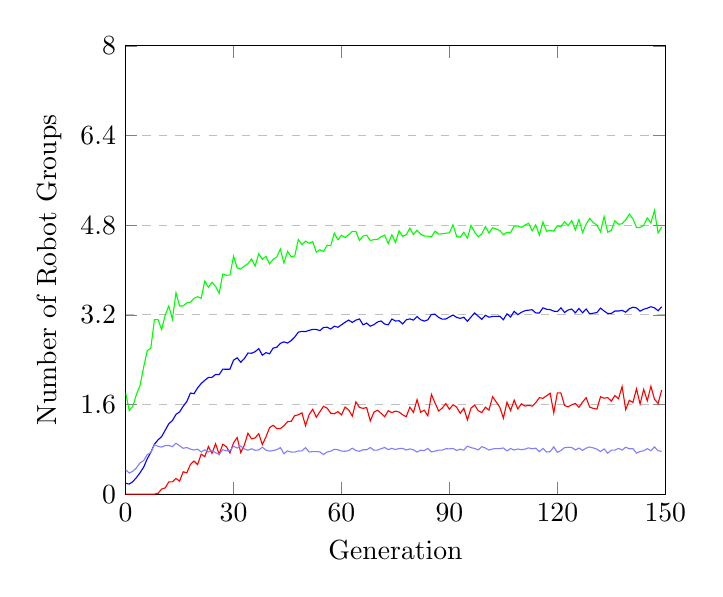
\begin{tikzpicture}
\begin{axis}[
	xlabel={Generation},
	ylabel={Number of Robot Groups},
	xmin=0, xmax=150,
	ymin=0, ymax=8,
	xtick={0.0,30.0,60.0,90.0,120.0,150.0},
	ytick={0.0,1.6,3.2,4.800000000000001,6.4,8.0},
	ymajorgrids=true,
	grid style=dashed,
]

\addplot[
	color=green,
	]
	coordinates {
	(0,1.8112499999999998)(1,1.4883333333333333)(2,1.5699166666666668)(3,1.7775833333333335)(4,1.9388333333333334)(5,2.2637500000000004)(6,2.5589999999999997)(7,2.606583333333334)(8,3.114)(9,3.1134166666666663)(10,2.9369999999999994)(11,3.1944166666666667)(12,3.3585833333333333)(13,3.1220000000000008)(14,3.5927499999999997)(15,3.356416666666666)(16,3.3581666666666674)(17,3.41125)(18,3.426916666666667)(19,3.4939999999999998)(20,3.523083333333334)(21,3.49575)(22,3.80425)(23,3.6916666666666664)(24,3.7808333333333333)(25,3.70625)(26,3.585666666666666)(27,3.9263333333333335)(28,3.9061666666666666)(29,3.909083333333333)(30,4.246166666666666)(31,4.036583333333334)(32,4.01775)(33,4.068916666666667)(34,4.1137500000000005)(35,4.197916666666667)(36,4.069583333333334)(37,4.290666666666667)(38,4.189083333333333)(39,4.243083333333333)(40,4.109416666666666)(41,4.1890833333333335)(42,4.229500000000001)(43,4.3743333333333325)(44,4.125083333333333)(45,4.332083333333333)(46,4.234666666666667)(47,4.248583333333333)(48,4.543916666666665)(49,4.4525)(50,4.514583333333333)(51,4.476249999999999)(52,4.505833333333333)(53,4.317833333333333)(54,4.361166666666667)(55,4.330333333333334)(56,4.441916666666667)(57,4.433249999999999)(58,4.655833333333333)(59,4.539833333333333)(60,4.6185)(61,4.580666666666667)(62,4.627916666666666)(63,4.687583333333333)(64,4.689416666666667)(65,4.52475)(66,4.607083333333333)(67,4.620083333333334)(68,4.52625)(69,4.540666666666667)(70,4.545333333333333)(71,4.593250000000001)(72,4.621583333333332)(73,4.472416666666667)(74,4.628166666666667)(75,4.4896666666666665)(76,4.698666666666667)(77,4.600833333333333)(78,4.628833333333333)(79,4.745666666666667)(80,4.630166666666667)(81,4.708333333333333)(82,4.638999999999999)(83,4.605666666666667)(84,4.604000000000001)(85,4.589333333333333)(86,4.693)(87,4.638916666666666)(88,4.646583333333334)(89,4.655083333333334)(90,4.663500000000001)(91,4.805333333333333)(92,4.600833333333334)(93,4.582999999999999)(94,4.673)(95,4.568416666666667)(96,4.7945)(97,4.677416666666667)(98,4.591583333333333)(99,4.643583333333334)(100,4.774666666666666)(101,4.659416666666667)(102,4.7535)(103,4.731833333333334)(104,4.704416666666667)(105,4.6291666666666655)(106,4.669999999999999)(107,4.667583333333334)(108,4.7828333333333335)(109,4.785083333333334)(110,4.761)(111,4.80075)(112,4.834)(113,4.697166666666666)(114,4.804749999999999)(115,4.6189166666666654)(116,4.856)(117,4.692666666666667)(118,4.703833333333334)(119,4.695166666666667)(120,4.787666666666666)(121,4.7739166666666675)(122,4.8620833333333335)(123,4.791833333333333)(124,4.8806666666666665)(125,4.71275)(126,4.901)(127,4.668416666666667)(128,4.817500000000001)(129,4.9199166666666665)(130,4.8445)(131,4.7995833333333335)(132,4.6834999999999996)(133,4.95325)(134,4.672833333333333)(135,4.709333333333334)(136,4.87825)(137,4.8155833333333335)(138,4.824666666666666)(139,4.895333333333333)(140,4.997333333333333)(141,4.913666666666667)(142,4.757083333333334)(143,4.758250000000001)(144,4.795333333333335)(145,4.929666666666666)(146,4.840583333333333)(147,5.060916666666667)(148,4.662833333333333)(149,4.767666666666667)
	};
\addplot[
	color=blue,
	]
	coordinates {
	(0,0.19299652777777782)(1,0.17928819444444444)(2,0.22347222222222224)(3,0.295173611111111)(4,0.3819965277777779)(5,0.4799444444444444)(6,0.6285729166666667)(7,0.7471840277777777)(8,0.8907916666666668)(9,0.9682708333333332)(10,1.0250277777777779)(11,1.1406458333333336)(12,1.2550520833333332)(13,1.3132881944444443)(14,1.4234166666666668)(15,1.4682465277777776)(16,1.568104166666667)(17,1.6521215277777783)(18,1.803194444444444)(19,1.792659722222222)(20,1.894850694444445)(21,1.9745625)(22,2.031288194444444)(23,2.0819270833333334)(24,2.083302083333333)(25,2.135090277777778)(26,2.1326944444444442)(27,2.2307187500000003)(28,2.227381944444444)(29,2.2296597222222223)(30,2.390697916666667)(31,2.432180555555556)(32,2.3540208333333332)(33,2.418875)(34,2.517871527777777)(35,2.5139201388888885)(36,2.5413680555555556)(37,2.5972222222222223)(38,2.4790590277777778)(39,2.5252534722222224)(40,2.5046597222222218)(41,2.605913194444445)(42,2.619944444444444)(43,2.6898958333333325)(44,2.7179374999999997)(45,2.6957881944444444)(46,2.7396909722222222)(47,2.8026770833333337)(48,2.890284722222222)(49,2.90470486111111)(50,2.9001909722222217)(51,2.9227222222222218)(52,2.938989583333333)(53,2.93857638888889)(54,2.918708333333334)(55,2.9733229166666666)(56,2.9788749999999995)(57,2.9454166666666666)(58,2.9969236111111113)(59,2.977611111111111)(60,3.0213194444444444)(61,3.066979166666667)(62,3.1056006944444445)(63,3.064673611111111)(64,3.104708333333333)(65,3.1255798611111114)(66,3.0209131944444447)(67,3.052635416666667)(68,2.996732638888889)(69,3.024204861111111)(70,3.0708819444444444)(71,3.0905104166666666)(72,3.0353055555555555)(73,3.021381944444445)(74,3.1250451388888885)(75,3.0890451388888884)(76,3.0940833333333333)(77,3.0376284722222215)(78,3.1112881944444446)(79,3.127586805555555)(80,3.1058402777777787)(81,3.1686493055555554)(82,3.1124930555555554)(83,3.0874930555555555)(84,3.110128472222222)(85,3.2087291666666666)(86,3.2091423611111107)(87,3.153013888888889)(88,3.1225590277777777)(89,3.1252777777777774)(90,3.161770833333334)(91,3.1962256944444443)(92,3.1536944444444437)(93,3.136090277777777)(94,3.155684027777778)(95,3.084447916666667)(96,3.1607083333333335)(97,3.2330416666666664)(98,3.175111111111111)(99,3.1201145833333324)(100,3.192003472222222)(101,3.1569201388888883)(102,3.1710208333333334)(103,3.1721770833333327)(104,3.174121527777778)(105,3.1121979166666667)(106,3.217920138888889)(107,3.160163194444445)(108,3.2626562500000005)(109,3.202048611111111)(110,3.2445208333333335)(111,3.273170138888889)(112,3.2831840277777773)(113,3.2905868055555554)(114,3.2333402777777773)(115,3.2325694444444437)(116,3.3245069444444444)(117,3.2989375)(118,3.2920312500000004)(119,3.2653194444444447)(120,3.2588055555555555)(121,3.324472222222222)(122,3.2413125)(123,3.2854062500000007)(124,3.3031388888888884)(125,3.2346319444444447)(126,3.3125104166666666)(127,3.2354687499999994)(128,3.304604166666667)(129,3.215756944444444)(130,3.229385416666666)(131,3.2398159722222224)(132,3.3198854166666667)(133,3.2671979166666665)(134,3.2234340277777775)(135,3.2250555555555556)(136,3.267152777777778)(137,3.267336805555556)(138,3.279350694444444)(139,3.2458576388888885)(140,3.308291666666666)(141,3.3348368055555553)(142,3.323809027777778)(143,3.2657534722222232)(144,3.2991770833333334)(145,3.3183819444444445)(146,3.3441319444444444)(147,3.324878472222222)(148,3.272454861111111)(149,3.3434409722222225)
	};
\addplot[
	color=red,
	]
	coordinates {
	(0,0.0)(1,0.0)(2,0.0)(3,0.0)(4,0.0)(5,0.0)(6,0.0001666666666666667)(7,0.00075)(8,0.0001666666666666667)(9,0.014916666666666665)(10,0.09016666666666666)(11,0.11191666666666666)(12,0.21983333333333333)(13,0.21983333333333338)(14,0.27925000000000005)(15,0.23266666666666663)(16,0.3990833333333333)(17,0.37875)(18,0.5288333333333333)(19,0.5906666666666666)(20,0.5276666666666665)(21,0.7134999999999999)(22,0.6685833333333332)(23,0.8494166666666666)(24,0.7285833333333334)(25,0.8987499999999999)(26,0.7115833333333332)(27,0.8908333333333334)(28,0.8460833333333336)(29,0.7346666666666667)(30,0.9161666666666667)(31,1.01025)(32,0.7419999999999999)(33,0.8762500000000002)(34,1.0865833333333335)(35,0.9861666666666666)(36,1.0041666666666667)(37,1.0789166666666667)(38,0.8843333333333332)(39,1.0208333333333333)(40,1.1851666666666667)(41,1.2294166666666666)(42,1.1714166666666668)(43,1.1692500000000001)(44,1.2181666666666664)(45,1.29375)(46,1.299166666666667)(47,1.4020833333333333)(48,1.415083333333333)(49,1.451)(50,1.2209999999999999)(51,1.4185)(52,1.5135833333333333)(53,1.371333333333333)(54,1.471666666666667)(55,1.566916666666667)(56,1.536166666666667)(57,1.4438333333333333)(58,1.4345000000000003)(59,1.4722499999999998)(60,1.4145)(61,1.5535833333333335)(62,1.5025833333333332)(63,1.392)(64,1.6458333333333335)(65,1.5460833333333333)(66,1.53075)(67,1.5453333333333332)(68,1.3049166666666665)(69,1.46075)(70,1.4966666666666666)(71,1.4434166666666668)(72,1.38075)(73,1.4885833333333334)(74,1.4537500000000003)(75,1.4814166666666664)(76,1.4645833333333333)(77,1.4153333333333336)(78,1.3823333333333334)(79,1.5519166666666666)(80,1.4570833333333333)(81,1.6858333333333333)(82,1.4616666666666664)(83,1.4978333333333338)(84,1.397416666666667)(85,1.7789166666666665)(86,1.6257499999999998)(87,1.4835833333333335)(88,1.5353333333333334)(89,1.615916666666667)(90,1.5145833333333334)(91,1.5948333333333333)(92,1.5529166666666665)(93,1.4410833333333333)(94,1.532)(95,1.3249166666666667)(96,1.533666666666667)(97,1.5890000000000002)(98,1.49075)(99,1.454)(100,1.5519166666666668)(101,1.500333333333333)(102,1.7396666666666667)(103,1.6450833333333335)(104,1.5510833333333331)(105,1.3552500000000003)(106,1.6419166666666665)(107,1.4905833333333334)(108,1.6767499999999997)(109,1.520333333333333)(110,1.6118333333333335)(111,1.571333333333333)(112,1.5831666666666666)(113,1.5711666666666666)(114,1.6327500000000001)(115,1.7214166666666668)(116,1.7100833333333327)(117,1.7541666666666669)(118,1.8006666666666669)(119,1.4508333333333332)(120,1.8075833333333335)(121,1.8048333333333335)(122,1.5804166666666664)(123,1.55725)(124,1.594333333333333)(125,1.6187500000000001)(126,1.5489166666666665)(127,1.6428333333333336)(128,1.7210833333333333)(129,1.5515)(130,1.52925)(131,1.517083333333333)(132,1.7383333333333335)(133,1.7110833333333333)(134,1.72325)(135,1.660916666666667)(136,1.759)(137,1.7019999999999997)(138,1.9187499999999997)(139,1.508333333333333)(140,1.67475)(141,1.6352499999999999)(142,1.87975)(143,1.6071666666666666)(144,1.8687499999999997)(145,1.6660000000000001)(146,1.9250000000000003)(147,1.6944166666666662)(148,1.6178333333333332)(149,1.8573333333333333)
	};
\addplot[
	color=blue!50,
	]
	coordinates {
	(0,0.4349714837315217)(1,0.37678405560741407)(2,0.4080384116316903)(3,0.4682941697687786)(4,0.5576682052025294)(5,0.5972304650058557)(6,0.7049042744123702)(7,0.7402035430738638)(8,0.8804939395041719)(9,0.8529995173183615)(10,0.8387318957213636)(11,0.8671274412146678)(12,0.8670416888244715)(13,0.8478035036026884)(14,0.9089113845840286)(15,0.8630857816870144)(16,0.81801054079443)(17,0.8314688151574687)(18,0.8028460340528062)(19,0.7873102227616627)(20,0.8015347449018019)(21,0.7528610731866079)(22,0.7904781365907804)(23,0.7531221872682666)(24,0.7747438770499077)(25,0.7391520310008656)(26,0.7106521434699103)(27,0.7913809163977017)(28,0.772828378879553)(29,0.7750934512555703)(30,0.8544299146262972)(31,0.8220791082627386)(32,0.8567933464331446)(33,0.8067510336484405)(34,0.783643468929102)(35,0.8091115669254787)(36,0.7819911984164415)(37,0.788918122297482)(38,0.8377206017917523)(39,0.7854412368779637)(40,0.7672030341951729)(41,0.7781240082607699)(42,0.7928911233565756)(43,0.8304089744828423)(44,0.7217388503799946)(45,0.7703687652162354)(46,0.7515707640780772)(47,0.7497514135189192)(48,0.7699530600042296)(49,0.7714132022725709)(50,0.8305662221640926)(51,0.7518668525723561)(52,0.7588329278233876)(53,0.7599086024464956)(54,0.7539992633735433)(55,0.706201416976775)(56,0.7517414220801129)(57,0.7664314680392986)(58,0.8001456577139258)(59,0.7916281310244782)(60,0.7678425321073047)(61,0.7646752455304225)(62,0.7767884644790258)(63,0.8201441022524134)(64,0.7776884469327552)(65,0.7644201482259992)(66,0.7923080510715085)(67,0.7907560651902498)(68,0.8319787210371963)(69,0.7836120724771687)(70,0.7863913751513569)(71,0.8110291066818901)(72,0.8332264961146716)(73,0.7936356433342177)(74,0.8174774459143163)(75,0.7962907104469298)(76,0.8128678214984709)(77,0.816040029486629)(78,0.7870880745198354)(79,0.8075449478749992)(80,0.7921861317886862)(81,0.7511483945333868)(82,0.7846913247523255)(83,0.775920293363781)(84,0.8162458184679395)(85,0.7530080573532636)(86,0.767463305326324)(87,0.7856604115218261)(88,0.7852476713550367)(89,0.8100657431567885)(90,0.8081340381239592)(91,0.8152702365829814)(92,0.7791222355471347)(93,0.8024158003150041)(94,0.7857629996613553)(95,0.8562874341784416)(96,0.8293677083717153)(97,0.8155506778821414)(98,0.7888481786725416)(99,0.84666163567556)(100,0.8223664279187899)(101,0.7857599143656271)(102,0.8074395662018623)(103,0.8128112670191493)(104,0.8122770005652528)(105,0.8241957976617617)(106,0.7721435525697373)(107,0.8142711428100007)(108,0.7869250202131677)(109,0.8053055400939553)(110,0.7930834902198275)(111,0.8030035508522815)(112,0.8256871030966545)(113,0.8090532278872299)(114,0.821145950639863)(115,0.7589022972114876)(116,0.8157086293753941)(117,0.7513581709281592)(118,0.7579245836569987)(119,0.8442533395926023)(120,0.7454128729730221)(121,0.7782526710625337)(122,0.8288316755759431)(123,0.8362432713893635)(124,0.832069309313455)(125,0.7876974029906427)(126,0.8226905702945795)(127,0.7795288961471436)(128,0.8212958372321265)(129,0.8408732040200207)(130,0.8247906616615687)(131,0.8026120622775165)(132,0.75934649834064)(133,0.8065749826327222)(134,0.7312068272931029)(135,0.784870243847701)(136,0.7851281374947342)(137,0.8163603076122016)(138,0.7852377252553653)(139,0.8379806555169952)(140,0.809275081277178)(141,0.8123471100550482)(142,0.73093964832055)(143,0.7617977785861593)(144,0.7735568430652336)(145,0.8112590238781691)(146,0.7750101219852813)(147,0.842556619001748)(148,0.7739987906249466)(149,0.7629644496051018)
	};
\end{axis}
\end{tikzpicture}
}
		\caption{Some sample caption}
		\label{fig:number-of-groups-easy}
	\end{subfigure}%
}
\\
\\
\\
\\
	\makebox[\linewidth][c]{%
	\begin{subfigure}[b]{0.7\textwidth}
		\centering
		\resizebox{0.9\linewidth}{!}{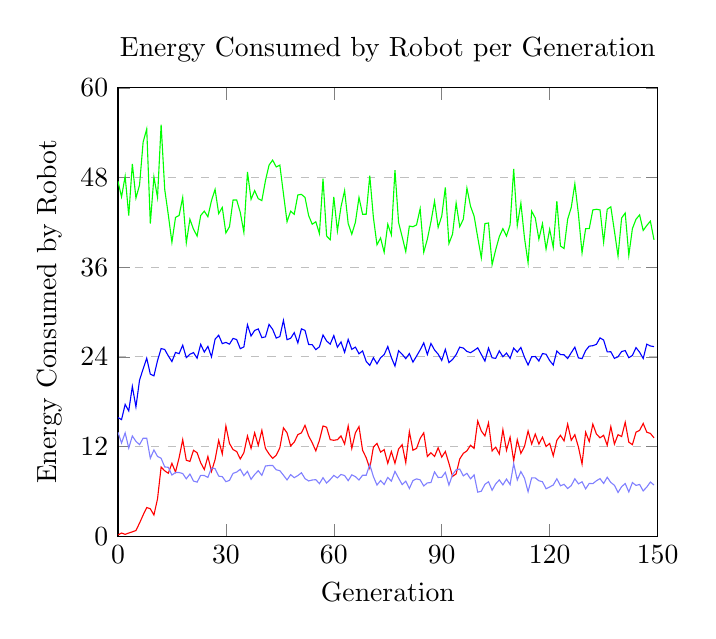
\begin{tikzpicture}
\begin{axis}[
	title={Energy Consumed by Robot per Generation},
	xlabel={Generation},
	ylabel={Energy Consumed by Robot},
	xmin=0, xmax=150,
	ymin=0, ymax=60,
	xtick={0.0,30.0,60.0,90.0,120.0,150.0},
	ytick={0.0,12.0,24.0,36.0,48.0,60.0},
	ymajorgrids=true,
	grid style=dashed,
]

\addplot[
	color=green,
	]
	coordinates {
	(0,47.5)(1,45.416666666666664)(2,48.166666666666664)(3,42.916666666666664)(4,49.833333333333336)(5,45.25)(6,47.00000000000001)(7,52.75)(8,54.50000000000001)(9,41.833333333333336)(10,48.083333333333336)(11,45.33333333333333)(12,55.083333333333336)(13,46.41666666666667)(14,43.0)(15,39.333333333333336)(16,42.666666666666664)(17,42.916666666666664)(18,45.333333333333336)(19,39.25)(20,42.41666666666667)(21,41.08333333333333)(22,40.166666666666664)(23,42.91666666666667)(24,43.5)(25,42.75)(26,44.916666666666664)(27,46.41666666666667)(28,43.16666666666667)(29,44.0)(30,40.583333333333336)(31,41.41666666666667)(32,44.99999999999999)(33,44.99999999999999)(34,43.333333333333336)(35,40.666666666666664)(36,48.75)(37,45.083333333333336)(38,46.25000000000001)(39,45.16666666666667)(40,44.91666666666667)(41,47.583333333333336)(42,49.666666666666664)(43,50.333333333333336)(44,49.41666666666667)(45,49.666666666666664)(46,45.83333333333333)(47,42.08333333333333)(48,43.5)(49,43.083333333333336)(50,45.66666666666667)(51,45.75)(52,45.333333333333336)(53,42.916666666666664)(54,41.75000000000001)(55,42.083333333333336)(56,40.5)(57,47.833333333333336)(58,40.16666666666667)(59,39.66666666666667)(60,45.416666666666664)(61,40.833333333333336)(62,44.083333333333336)(63,46.25)(64,41.833333333333336)(65,40.416666666666664)(66,42.0)(67,45.333333333333336)(68,43.08333333333333)(69,43.083333333333336)(70,48.25)(71,42.66666666666667)(72,39.0)(73,39.916666666666664)(74,38.0)(75,41.75)(76,40.333333333333336)(77,49.0)(78,41.99999999999999)(79,40.083333333333336)(80,38.08333333333333)(81,41.49999999999999)(82,41.41666666666667)(83,41.666666666666664)(84,43.83333333333333)(85,38.0)(86,39.75)(87,42.08333333333333)(88,44.833333333333336)(89,41.333333333333336)(90,42.83333333333333)(91,46.666666666666664)(92,39.16666666666667)(93,40.416666666666664)(94,44.583333333333336)(95,41.416666666666664)(96,42.416666666666664)(97,46.58333333333333)(98,44.166666666666664)(99,42.83333333333333)(100,40.0)(101,37.25)(102,41.833333333333336)(103,41.916666666666664)(104,36.333333333333336)(105,38.333333333333336)(106,40.083333333333336)(107,41.16666666666667)(108,40.166666666666664)(109,41.66666666666667)(110,49.166666666666664)(111,41.583333333333336)(112,44.583333333333336)(113,39.916666666666664)(114,36.583333333333336)(115,43.5)(116,42.583333333333336)(117,39.75)(118,41.83333333333333)(119,38.41666666666667)(120,41.08333333333333)(121,38.666666666666664)(122,44.833333333333336)(123,38.83333333333333)(124,38.5)(125,42.41666666666667)(126,44.0)(127,47.166666666666664)(128,43.08333333333333)(129,37.91666666666667)(130,41.166666666666664)(131,41.166666666666664)(132,43.666666666666664)(133,43.75000000000001)(134,43.666666666666664)(135,39.33333333333333)(136,43.75)(137,44.08333333333333)(138,40.833333333333336)(139,37.5)(140,42.583333333333336)(141,43.25)(142,37.583333333333336)(143,41.16666666666667)(144,42.41666666666667)(145,43.0)(146,40.916666666666664)(147,41.58333333333333)(148,42.166666666666664)(149,39.666666666666664)
	};
\addplot[
	color=blue,
	]
	coordinates {
	(0,15.875)(1,15.600694444444445)(2,17.631944444444443)(3,16.767361111111114)(4,20.038194444444446)(5,17.305555555555554)(6,20.87847222222222)(7,22.38888888888889)(8,23.812499999999996)(9,21.684027777777782)(10,21.458333333333336)(11,23.5)(12,25.11111111111111)(13,24.986111111111114)(14,24.128472222222218)(15,23.36805555555555)(16,24.59027777777778)(17,24.430555555555554)(18,25.559027777777782)(19,23.895833333333336)(20,24.34722222222222)(21,24.572916666666668)(22,23.81944444444445)(23,25.677083333333332)(24,24.642361111111114)(25,25.395833333333336)(26,24.0)(27,26.364583333333336)(28,26.892361111111114)(29,25.77430555555556)(30,25.930555555555557)(31,25.70486111111111)(32,26.46527777777778)(33,26.315972222222225)(34,25.093750000000004)(35,25.32638888888889)(36,28.29861111111111)(37,26.791666666666664)(38,27.53472222222222)(39,27.73611111111111)(40,26.569444444444443)(41,26.677083333333332)(42,28.34027777777778)(43,27.680555555555557)(44,26.517361111111114)(45,26.71875)(46,28.874999999999996)(47,26.29861111111111)(48,26.486111111111114)(49,27.239583333333332)(50,25.864583333333336)(51,27.75)(52,27.538194444444443)(53,25.65972222222222)(54,25.624999999999996)(55,24.965277777777775)(56,25.34375)(57,26.923611111111114)(58,26.12152777777778)(59,25.701388888888886)(60,26.850694444444443)(61,25.29513888888889)(62,25.99652777777778)(63,24.60763888888889)(64,26.333333333333332)(65,25.00347222222222)(66,25.305555555555557)(67,24.40972222222222)(68,24.795138888888893)(69,23.392361111111107)(70,22.85416666666667)(71,23.885416666666664)(72,23.069444444444443)(73,23.875)(74,24.302083333333332)(75,25.381944444444446)(76,23.90277777777778)(77,22.770833333333336)(78,24.81597222222222)(79,24.354166666666664)(80,23.756944444444443)(81,24.4375)(82,23.291666666666664)(83,24.100694444444443)(84,24.927083333333332)(85,25.864583333333332)(86,24.315972222222218)(87,25.795138888888893)(88,24.920138888888893)(89,24.364583333333332)(90,23.517361111111114)(91,25.006944444444443)(92,23.23263888888889)(93,23.645833333333336)(94,24.295138888888886)(95,25.302083333333332)(96,25.177083333333332)(97,24.72916666666667)(98,24.555555555555557)(99,24.857638888888886)(100,25.20833333333333)(101,24.32638888888889)(102,23.43402777777778)(103,25.177083333333332)(104,23.87847222222222)(105,23.798611111111114)(106,24.80208333333333)(107,24.017361111111114)(108,24.510416666666668)(109,23.802083333333336)(110,25.163194444444446)(111,24.631944444444446)(112,25.260416666666668)(113,23.947916666666664)(114,22.913194444444446)(115,24.010416666666664)(116,24.045138888888886)(117,23.44097222222222)(118,24.440972222222225)(119,24.354166666666664)(120,23.503472222222225)(121,22.909722222222218)(122,24.784722222222225)(123,24.312499999999996)(124,24.274305555555557)(125,23.770833333333332)(126,24.55902777777778)(127,25.298611111111114)(128,23.864583333333336)(129,23.76041666666667)(130,24.836805555555557)(131,25.43402777777778)(132,25.493055555555554)(133,25.680555555555557)(134,26.53819444444444)(135,26.246527777777775)(136,24.67013888888889)(137,24.680555555555557)(138,23.79861111111111)(139,24.01041666666667)(140,24.71875)(141,24.836805555555557)(142,23.88888888888889)(143,24.1875)(144,25.23611111111111)(145,24.62152777777778)(146,23.781250000000004)(147,25.701388888888893)(148,25.458333333333332)(149,25.368055555555557)
	};
\addplot[
	color=red,
	]
	coordinates {
	(0,0.16666666666666666)(1,0.41666666666666663)(2,0.25)(3,0.41666666666666663)(4,0.5833333333333333)(5,0.75)(6,1.75)(7,2.8333333333333335)(8,3.8333333333333335)(9,3.666666666666667)(10,2.833333333333333)(11,5.0)(12,9.25)(13,8.75)(14,8.416666666666666)(15,9.75)(16,8.583333333333334)(17,10.5)(18,12.916666666666666)(19,10.166666666666666)(20,10.0)(21,11.5)(22,11.166666666666666)(23,9.833333333333332)(24,8.916666666666666)(25,10.666666666666668)(26,8.666666666666666)(27,10.25)(28,12.833333333333334)(29,11.0)(30,14.75)(31,12.416666666666668)(32,11.583333333333334)(33,11.333333333333334)(34,10.333333333333332)(35,11.166666666666666)(36,13.416666666666668)(37,11.75)(38,13.833333333333334)(39,12.166666666666666)(40,14.166666666666666)(41,11.75)(42,11.0)(43,10.416666666666666)(44,10.833333333333332)(45,11.833333333333332)(46,14.5)(47,13.833333333333332)(48,12.083333333333332)(49,12.583333333333334)(50,13.583333333333332)(51,13.833333333333334)(52,14.833333333333334)(53,13.416666666666666)(54,12.5)(55,11.416666666666668)(56,12.833333333333334)(57,14.749999999999998)(58,14.583333333333334)(59,12.916666666666668)(60,12.833333333333334)(61,12.916666666666666)(62,13.416666666666668)(63,12.333333333333334)(64,14.749999999999998)(65,11.749999999999998)(66,13.833333333333334)(67,14.666666666666668)(68,11.5)(69,10.5)(70,9.083333333333334)(71,11.916666666666666)(72,12.416666666666668)(73,11.25)(74,11.583333333333334)(75,9.749999999999998)(76,11.333333333333334)(77,9.75)(78,11.666666666666668)(79,12.249999999999998)(80,9.833333333333334)(81,13.999999999999998)(82,11.5)(83,11.749999999999998)(84,13.083333333333332)(85,13.833333333333332)(86,10.666666666666666)(87,11.166666666666666)(88,10.666666666666668)(89,11.833333333333334)(90,10.583333333333332)(91,11.333333333333334)(92,9.75)(93,7.999999999999999)(94,8.333333333333334)(95,10.333333333333332)(96,11.083333333333332)(97,11.416666666666666)(98,12.166666666666666)(99,11.75)(100,15.416666666666668)(101,14.083333333333334)(102,13.416666666666666)(103,15.166666666666666)(104,11.416666666666666)(105,11.916666666666666)(106,11.0)(107,14.249999999999998)(108,11.5)(109,13.250000000000002)(110,10.083333333333334)(111,12.916666666666668)(112,11.083333333333334)(113,12.0)(114,14.083333333333332)(115,12.333333333333334)(116,13.666666666666666)(117,12.333333333333332)(118,13.249999999999998)(119,11.999999999999998)(120,12.416666666666666)(121,10.750000000000002)(122,12.833333333333334)(123,13.500000000000002)(124,12.749999999999998)(125,15.0)(126,12.833333333333334)(127,13.583333333333334)(128,11.916666666666666)(129,9.666666666666666)(130,13.916666666666664)(131,12.666666666666666)(132,15.000000000000002)(133,13.666666666666666)(134,13.166666666666668)(135,13.499999999999998)(136,12.166666666666666)(137,14.666666666666666)(138,12.333333333333334)(139,13.583333333333332)(140,13.333333333333334)(141,15.25)(142,12.583333333333334)(143,12.25)(144,13.916666666666664)(145,14.166666666666666)(146,15.083333333333334)(147,13.916666666666668)(148,13.749999999999998)(149,13.166666666666668)
	};
\addplot[
	color=blue!50,
	]
	coordinates {
	(0,13.90267508831089)(1,12.47226672500314)(2,13.829624590349557)(3,11.789274573223636)(4,13.413844666176374)(5,12.688883505652079)(6,12.257167226349628)(7,13.106379522748576)(8,13.110225882701092)(9,10.426841176890743)(10,11.545012687873774)(11,10.67171785150359)(12,10.424450249766346)(13,9.265681375173264)(14,9.216473419020714)(15,8.18516134471119)(16,8.515399246235402)(17,8.520171334785168)(18,8.384822908560828)(19,7.6774441419309625)(20,8.313776502588945)(21,7.383943844763538)(22,7.226351019568069)(23,8.14228601526083)(24,8.120382544078307)(25,7.864600729350112)(26,9.128590844517353)(27,9.036741475390718)(28,8.037961055029903)(29,7.966856790838541)(30,7.299041024437335)(31,7.464516831172022)(32,8.40847260936773)(33,8.579220170591192)(34,8.958164879835902)(35,8.104103361144595)(36,8.675555453991384)(37,7.604493560433139)(38,8.26013414114198)(39,8.761153843912247)(40,8.139475024194684)(41,9.390051821918272)(42,9.456435175042492)(43,9.467155038754942)(44,8.884298136861146)(45,8.765882660828167)(46,8.160842619939334)(47,7.529402918218205)(48,8.23719682195419)(49,7.829660062721458)(50,8.107746091565126)(51,8.486096268382749)(52,7.703726537669015)(53,7.38905924607209)(54,7.518516882515916)(55,7.5622872574268545)(56,7.0341639126835975)(57,7.826614501890382)(58,7.107693029436927)(59,7.57718604891149)(60,8.133221119978028)(61,7.799516914047528)(62,8.262157162117933)(63,8.112632253380381)(64,7.428536064132439)(65,8.20771428378926)(66,7.964761511693097)(67,7.521830821678718)(68,8.158001693026549)(69,8.160197053607996)(70,9.586478122984042)(71,7.9803460395866885)(72,6.846341369349167)(73,7.444256782802697)(74,6.920720916403518)(75,7.860331642475469)(76,7.366497370163017)(77,8.670466769779681)(78,7.777506107446994)(79,6.903838564445453)(80,7.35614985562651)(81,6.384405180049235)(82,7.4438595473128455)(83,7.671165252945963)(84,7.539413194921626)(85,6.720120552922453)(86,7.130831208411188)(87,7.172999931789191)(88,8.606450347921854)(89,7.857038781391409)(90,7.8778203960473725)(91,8.539956688965365)(92,6.83866536730472)(93,8.22220527383319)(94,8.888584015865774)(95,8.98686113162109)(96,8.070860893944689)(97,8.414012067462812)(98,7.674393348379541)(99,8.202483047272889)(100,5.889440699055045)(101,6.020486835739401)(102,6.936682403265805)(103,7.285110867790616)(104,6.14522944810159)(105,7.002938325618786)(106,7.532862750630825)(107,6.8635942184122065)(108,7.644630681967605)(109,6.897340718388838)(110,9.719004561105358)(111,7.521371653077291)(112,8.646030969845379)(113,7.763144800383364)(114,5.946528149668643)(115,7.806759264864431)(116,7.80524377897229)(117,7.419492711009111)(118,7.285768141969099)(119,6.342404244214291)(120,6.586610616391859)(121,6.848151449808877)(122,7.686711128937212)(123,6.742661657630832)(124,6.940591169370634)(125,6.3826841034697175)(126,6.771104115378577)(127,7.682793579809095)(128,7.003504145793773)(129,7.278668913007887)(130,6.329037875691446)(131,7.066771096257844)(132,7.0322988790245855)(133,7.416565840293636)(134,7.702236216427049)(135,7.05317767586283)(136,7.885177271954002)(137,7.1902223963047796)(138,6.811278373303489)(139,5.8421893515899)(140,6.624523656584128)(141,7.0445051765022)(142,5.916024314177142)(143,7.178376729674846)(144,6.794461522518879)(145,6.921970051556661)(146,6.055792718647465)(147,6.577610085427416)(148,7.244686210467727)(149,6.843831608522187)
	};
\end{axis}
\end{tikzpicture}
}
		\caption{Some sample caption}
		\label{fig:energy-consumed-by-robot-easy}
	\end{subfigure}%
	\begin{subfigure}[b]{0.7\textwidth}
		\centering
		\resizebox{0.9\linewidth}{!}{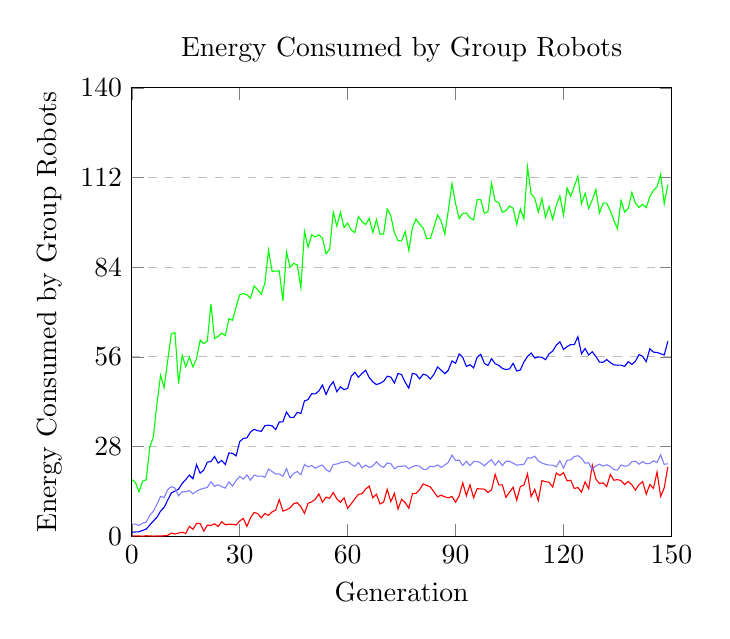
\begin{tikzpicture}
\begin{axis}[
	title={Energy Consumed by Group Robots},
	xlabel={Generation},
	ylabel={Energy Consumed by Group Robots},
	xmin=0, xmax=150,
	ymin=0, ymax=140,
	xtick={0.0,30.0,60.0,90.0,120.0,150.0},
	ytick={0.0,28.0,56.0,84.0,112.0,140.0},
	ymajorgrids=true,
	grid style=dashed,
]

\addplot[
	color=green,
	]
	coordinates {
	(0,17.666666666666664)(1,16.805555555555557)(2,13.861111111111109)(3,17.194444444444446)(4,17.583333333333332)(5,27.72222222222222)(6,31.055555555555554)(7,41.49999999999999)(8,50.222222222222214)(9,46.416666666666664)(10,54.972222222222214)(11,63.19444444444444)(12,63.55555555555555)(13,47.69444444444445)(14,56.55555555555556)(15,52.888888888888886)(16,55.972222222222214)(17,52.833333333333336)(18,55.49999999999999)(19,61.22222222222223)(20,60.111111111111114)(21,60.97222222222222)(22,72.55555555555554)(23,61.72222222222222)(24,62.388888888888886)(25,63.361111111111114)(26,62.61111111111111)(27,67.91666666666667)(28,67.41666666666666)(29,71.6111111111111)(30,75.3888888888889)(31,75.77777777777777)(32,75.38888888888889)(33,74.33333333333334)(34,78.16666666666666)(35,76.94444444444444)(36,75.58333333333334)(37,78.99999999999999)(38,89.38888888888889)(39,82.69444444444444)(40,82.77777777777779)(41,82.83333333333333)(42,73.47222222222221)(43,88.75)(44,83.94444444444444)(45,85.19444444444446)(46,84.69444444444443)(47,77.52777777777777)(48,95.16666666666667)(49,90.25)(50,94.13888888888887)(51,93.47222222222223)(52,94.11111111111111)(53,93.02777777777777)(54,88.19444444444443)(55,89.61111111111113)(56,101.22222222222223)(57,96.80555555555556)(58,101.11111111111113)(59,96.38888888888887)(60,97.77777777777779)(61,95.58333333333334)(62,94.80555555555554)(63,99.80555555555554)(64,98.27777777777777)(65,97.30555555555556)(66,99.25000000000001)(67,94.83333333333333)(68,98.88888888888889)(69,94.27777777777777)(70,94.38888888888891)(71,102.19444444444444)(72,100.05555555555556)(73,94.69444444444443)(74,92.27777777777779)(75,92.19444444444444)(76,95.11111111111113)(77,89.19444444444446)(78,96.30555555555556)(79,99.00000000000001)(80,97.41666666666666)(81,96.2222222222222)(82,92.88888888888887)(83,93.0)(84,96.5)(85,100.30555555555556)(86,98.41666666666666)(87,94.30555555555554)(88,101.83333333333333)(89,110.08333333333331)(90,103.8888888888889)(91,99.16666666666666)(92,100.75000000000001)(93,100.94444444444447)(94,99.38888888888889)(95,98.74999999999999)(96,105.11111111111111)(97,105.1111111111111)(98,100.83333333333334)(99,101.3611111111111)(100,110.19444444444443)(101,104.72222222222221)(102,104.16666666666667)(103,101.16666666666666)(104,101.6388888888889)(105,103.11111111111111)(106,102.44444444444444)(107,97.41666666666667)(108,102.16666666666667)(109,99.08333333333334)(110,115.30555555555556)(111,106.86111111111113)(112,105.61111111111111)(113,101.16666666666664)(114,105.41666666666667)(115,99.55555555555556)(116,102.94444444444444)(117,98.94444444444443)(118,103.3888888888889)(119,106.27777777777779)(120,100.22222222222221)(121,108.75)(122,106.13888888888889)(123,109.25)(124,112.3888888888889)(125,103.74999999999999)(126,107.08333333333333)(127,102.3888888888889)(128,105.05555555555556)(129,108.30555555555554)(130,100.91666666666667)(131,103.99999999999999)(132,104.0)(133,101.61111111111111)(134,98.61111111111109)(135,96.02777777777779)(136,104.88888888888887)(137,101.19444444444443)(138,102.36111111111111)(139,107.30555555555553)(140,103.9722222222222)(141,102.69444444444444)(142,103.63888888888889)(143,102.58333333333334)(144,106.05555555555554)(145,107.99999999999999)(146,109.08333333333333)(147,113.02777777777776)(148,103.80555555555557)(149,109.77777777777779)
	};
\addplot[
	color=blue,
	]
	coordinates {
	(0,1.204861111111111)(1,1.3310185185185184)(2,1.378472222222222)(3,1.804398148148148)(4,2.204861111111112)(5,3.4837962962962967)(6,4.756944444444445)(7,5.918981481481482)(8,7.8402777777777795)(9,9.03125)(10,11.315972222222223)(11,13.51273148148148)(12,14.090277777777779)(13,14.658564814814815)(14,16.48611111111111)(15,17.672453703703706)(16,19.08101851851852)(17,17.960648148148145)(18,22.34027777777778)(19,19.663194444444446)(20,20.63888888888889)(21,23.10416666666667)(22,23.297453703703706)(23,24.890046296296294)(24,22.835648148148152)(25,23.644675925925924)(26,22.37615740740741)(27,25.99652777777778)(28,25.868055555555554)(29,25.077546296296294)(30,29.55439814814815)(31,30.521990740740744)(32,30.71412037037037)(33,32.55324074074074)(34,33.363425925925924)(35,32.949074074074076)(36,32.7349537037037)(37,34.520833333333336)(38,34.68287037037037)(39,34.45370370370371)(40,33.32175925925926)(41,35.64699074074074)(42,35.71527777777778)(43,38.78935185185185)(44,37.10300925925927)(45,37.1099537037037)(46,38.645833333333336)(47,38.33101851851852)(48,42.25000000000001)(49,42.65740740740741)(50,44.482638888888886)(51,44.447916666666664)(52,45.34606481481481)(53,47.214120370370374)(54,44.24189814814814)(55,46.739583333333336)(56,48.23148148148148)(57,45.12847222222222)(58,46.646990740740755)(59,45.75810185185185)(60,46.15625)(61,49.954861111111114)(62,51.19444444444445)(63,49.61689814814814)(64,50.81944444444444)(65,51.81944444444444)(66,49.55671296296297)(67,48.186342592592595)(68,47.34837962962963)(69,47.741898148148145)(70,48.351851851851855)(71,49.954861111111114)(72,49.682870370370374)(73,47.8125)(74,50.79398148148147)(75,50.451388888888886)(76,48.05902777777777)(77,46.22222222222223)(78,50.84606481481481)(79,50.58796296296296)(80,49.10532407407407)(81,50.60069444444444)(82,50.2361111111111)(83,49.101851851851855)(84,50.563657407407405)(85,52.86574074074075)(86,51.83912037037037)(87,50.74768518518519)(88,51.863425925925924)(89,54.730324074074076)(90,53.97800925925925)(91,56.90393518518519)(92,55.85416666666667)(93,52.98495370370371)(94,53.53819444444444)(95,52.56018518518518)(96,55.87731481481482)(97,56.79513888888888)(98,53.95949074074074)(99,53.29629629629629)(100,55.44907407407408)(101,53.8599537037037)(102,53.36805555555556)(103,52.383101851851855)(104,52.04050925925925)(105,52.24884259259259)(106,53.97569444444444)(107,51.57754629629629)(108,51.91203703703703)(109,54.4212962962963)(110,56.13773148148148)(111,57.211805555555564)(112,55.63773148148149)(113,55.97222222222223)(114,55.864583333333336)(115,55.12268518518518)(116,56.9699074074074)(117,57.80439814814815)(118,59.67476851851852)(119,60.68055555555556)(120,58.32175925925926)(121,59.19907407407407)(122,59.83564814814815)(123,59.8425925925926)(124,62.28356481481481)(125,56.949074074074076)(126,58.60416666666666)(127,56.5787037037037)(128,57.599537037037045)(129,56.1087962962963)(130,54.38310185185185)(131,54.28356481481482)(132,55.164351851851855)(133,54.208333333333336)(134,53.51273148148148)(135,53.39467592592593)(136,53.41782407407407)(137,53.00694444444445)(138,54.50462962962962)(139,53.63425925925926)(140,54.644675925925924)(141,56.69560185185185)(142,56.158564814814824)(143,54.5173611111111)(144,58.54050925925927)(145,57.48263888888889)(146,57.375)(147,56.98148148148148)(148,56.581018518518526)(149,60.862268518518526)
	};
\addplot[
	color=red,
	]
	coordinates {
	(0,0.027777777777777776)(1,0.1111111111111111)(2,0.08333333333333333)(3,0.0)(4,0.1388888888888889)(5,0.08333333333333333)(6,0.027777777777777776)(7,0.08333333333333333)(8,0.05555555555555555)(9,0.1388888888888889)(10,0.25)(11,1.0)(12,0.6666666666666667)(13,0.9722222222222222)(14,1.222222222222222)(15,0.888888888888889)(16,3.083333333333333)(17,2.166666666666666)(18,4.0)(19,3.9722222222222214)(20,1.6111111111111112)(21,3.4166666666666665)(22,3.3888888888888884)(23,3.861111111111111)(24,3.0277777777777777)(25,4.5)(26,3.5277777777777777)(27,3.75)(28,3.7222222222222223)(29,3.472222222222222)(30,4.75)(31,5.555555555555555)(32,3.055555555555556)(33,5.777777777777778)(34,7.416666666666667)(35,7.083333333333334)(36,5.722222222222221)(37,7.083333333333333)(38,6.5)(39,7.583333333333332)(40,8.138888888888888)(41,11.416666666666666)(42,7.833333333333334)(43,8.25)(44,8.833333333333332)(45,10.166666666666668)(46,10.444444444444445)(47,9.222222222222221)(48,7.111111111111112)(49,10.277777777777779)(50,10.722222222222221)(51,11.555555555555557)(52,13.194444444444443)(53,10.611111111111112)(54,12.194444444444445)(55,11.833333333333336)(56,13.63888888888889)(57,11.61111111111111)(58,10.583333333333332)(59,11.972222222222221)(60,8.694444444444446)(61,10.13888888888889)(62,11.63888888888889)(63,13.083333333333332)(64,13.277777777777779)(65,14.722222222222221)(66,15.63888888888889)(67,12.0)(68,13.111111111111109)(69,10.055555555555554)(70,10.63888888888889)(71,14.63888888888889)(72,10.777777777777777)(73,13.361111111111112)(74,8.472222222222223)(75,11.527777777777779)(76,10.472222222222223)(77,8.722222222222223)(78,13.277777777777777)(79,13.36111111111111)(80,14.527777777777777)(81,16.333333333333332)(82,15.861111111111109)(83,15.361111111111112)(84,13.805555555555557)(85,12.277777777777779)(86,12.805555555555554)(87,12.277777777777779)(88,12.0)(89,12.416666666666668)(90,10.61111111111111)(91,12.63888888888889)(92,16.66666666666667)(93,12.638888888888891)(94,16.083333333333336)(95,11.999999999999998)(96,14.861111111111109)(97,14.750000000000002)(98,14.694444444444446)(99,13.666666666666666)(100,14.444444444444443)(101,19.305555555555557)(102,16.055555555555557)(103,16.0)(104,12.111111111111109)(105,13.777777777777777)(106,15.277777777777777)(107,11.222222222222223)(108,15.500000000000002)(109,15.972222222222221)(110,19.472222222222225)(111,12.333333333333332)(112,14.63888888888889)(113,11.11111111111111)(114,17.36111111111111)(115,17.02777777777778)(116,16.833333333333336)(117,15.333333333333332)(118,19.75)(119,18.97222222222223)(120,19.833333333333332)(121,17.277777777777775)(122,17.472222222222225)(123,14.888888888888891)(124,15.194444444444443)(125,13.75)(126,16.97222222222222)(127,14.805555555555555)(128,22.194444444444443)(129,17.833333333333332)(130,16.444444444444446)(131,16.666666666666668)(132,15.472222222222221)(133,19.277777777777775)(134,17.47222222222222)(135,17.666666666666664)(136,17.36111111111111)(137,16.13888888888889)(138,17.11111111111111)(139,16.055555555555554)(140,14.388888888888888)(141,16.11111111111111)(142,17.055555555555554)(143,13.111111111111112)(144,16.13888888888889)(145,14.944444444444445)(146,20.02777777777778)(147,12.416666666666668)(148,15.111111111111114)(149,21.611111111111114)
	};
\addplot[
	color=blue!50,
	]
	coordinates {
	(0,3.793637938766837)(1,3.7523379573637192)(2,3.328567501675064)(3,4.030622213270808)(4,4.4200511181489555)(5,6.519824814561398)(6,7.802042272417542)(7,10.02441977439477)(8,12.394071449676321)(9,12.103048049487064)(10,14.57959618435815)(11,15.485529877572361)(12,15.034668068213444)(13,12.603791535892713)(14,13.859131958019335)(15,13.893695320975688)(16,14.276972976489066)(17,13.22815768166678)(18,14.055143819485444)(19,14.622606430366234)(20,14.957302266366)(21,15.235080611643786)(22,17.010023256091696)(23,15.54041286278934)(24,16.06585257567348)(25,15.463743324103445)(26,15.017060927033821)(27,16.99920117965988)(28,15.638964693265052)(29,17.357328711496155)(30,18.65930225851148)(31,17.817017139874075)(32,19.15098610194967)(33,17.49211868808712)(34,19.07601101744591)(35,18.72609079639066)(36,18.781965227909247)(37,18.39148958131118)(38,20.990059804215992)(39,20.19393388085553)(40,19.42155311976079)(41,19.466427884989365)(42,18.674249766031945)(43,21.099624848741005)(44,18.18430051809181)(45,19.639222180868042)(46,20.186544048266615)(47,19.165787771049892)(48,22.406292112976733)(49,21.637076798051105)(50,22.07681205051556)(51,21.19582457976546)(52,21.81479580683102)(53,22.21874003690169)(54,20.751469937438127)(55,20.119478712936015)(56,22.390235817320768)(57,22.532265685785312)(58,22.94179252512627)(59,23.17790456840255)(60,23.374023837530512)(61,22.44264885088899)(62,21.797006412357266)(63,23.033471985534707)(64,21.33204072423209)(65,22.225328737529967)(66,21.463398849893995)(67,21.876051654403554)(68,23.254525487465227)(69,22.04178875176993)(70,21.486804029634754)(71,22.87804553388826)(72,22.6268344731064)(73,21.06987673238088)(74,21.77638873835049)(75,21.843403947318553)(76,21.99489900246392)(77,21.061199648796194)(78,21.733479954188343)(79,22.04848039440876)(80,21.860752690829468)(81,20.872231866412836)(82,20.87737121227454)(83,21.87810009551734)(84,21.649128015090245)(85,22.255461017226825)(86,21.481186985707282)(87,22.229964783114706)(88,23.019410518842715)(89,25.320192971512302)(90,23.640904586511194)(91,23.751498134614707)(92,22.074041947008315)(93,23.40618453196275)(94,22.06262937619204)(95,23.30364861466495)(96,23.367568507380653)(97,22.88888347001476)(98,21.9613032214439)(99,23.05656757258113)(100,23.8795828518469)(101,22.173941163138757)(102,23.555090297325638)(103,22.042569989096897)(104,23.387709176985048)(105,23.408034199414868)(106,22.822599314642197)(107,22.188003546626796)(108,22.318822499079342)(109,22.44671611165769)(110,24.41890101869657)(111,24.42938748046953)(112,24.995956868444676)(113,23.52914829444043)(114,22.84338416929849)(115,22.457801784008492)(116,22.17880289408619)(117,22.1752024655541)(118,21.66844593658571)(119,23.544065436336)(120,21.293477236817772)(121,23.699115144118934)(122,23.858499913315633)(123,24.876558087166273)(124,25.139259805821098)(125,24.370286751592847)(126,22.796628936785954)(127,22.945130761542615)(128,20.712334622816293)(129,22.02718560513645)(130,22.48307169661878)(131,21.892344889711108)(132,22.302944315019634)(133,21.785769583376787)(134,20.78000456681748)(135,20.681228909177996)(136,22.2383585400881)(137,21.85109005991582)(138,22.02406005363854)(139,23.27594489367388)(140,23.413843949583757)(141,22.489554217561924)(142,23.281602832734492)(143,22.636691631241852)(144,22.71564516555098)(145,23.537547512483464)(146,23.02467193574319)(147,25.40396907333671)(148,22.4235322956733)(149,22.629412830065373)
	};
\end{axis}
\end{tikzpicture}
}
		\caption{Some sample caption}
		\label{fig:energy-consumed-by-group-easy}
	\end{subfigure}%

}
\caption{Figure shows results from a simulation in the easy environment (p.2)}
\end{figure}
